\chapter{\textit{Phylum} Protozoa}
\section{\textit{Sarcodinia}}
\subsection{\textit{Entamoeba histolítica}}
Ameba cosmopolita, aunque con gran incidencia en regiones tropicales y subtropicales (prevalencia de hasta el 40 \%). Provoca, entre otras patologías, la \textit{diarrea del viajero}. Afecta a 10 millones de personas en todo el mundo, causando unas 100000 muertes anuales, siendo el 80 \% de los infectados portadores sanos. No obstante, la facilidad de confusión con \textit{Entamoeba dispar}, otra ameba comensal y no patógena, hace que los datos no sean del todo exactos. Se diferencian mediante técnicas de laboratorio (moleculares y bioquímicas).
\subsubsection{Morfología}
\textit{E. histolytica} presenta dos formas: una patógena (trofozoito) y otra de resistencia (quiste).
\begin{itemize}[itemsep=0pt,parsep=0pt,topsep=0pt,partopsep=0pt]
	\begin{multicols}{2}
		\item \textbf{Trofozoito}: (figura \ref{fig:PARASIT:EHistolyticaMorf}, derecha) sin forma constante por la emisión de pseudópodos, se meuve sobre superficies de forma directa por la emisión de lobópodos. Presenta dos zonas: ectoplasma (externo, de aspecto hialino y sin orgánulos celulares) y endoplasma (interno, rugoso y con orgánulos celulares). Tiene un núcleo con un nucleolo central y heterocromatina dispuesta perifericamente. En el citoplasma no se hallan mitocondrias, retículo endoplásmico o aparato de Golgi, pero sí polirribosomas, microtúbulos, glucógeno $\alpha \mbox{ o } \beta$ y vacuolas alimentarias con eritrocitos en degradación.
		\columnbreak
		\begin{figure}[H]
			\centering
			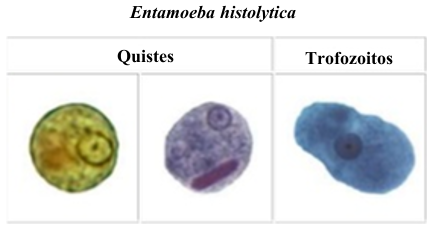
\includegraphics[width=0.9\columnwidth]{A.imagenes/ACV-BioSan-Parasit-EHistolyticaMorf}
			\caption[Quistes de \textit{E. Histolytica}]{\textit{E. histolytica} en sus dos morfologías: la de resistencia o quiste, con 2 ó 4 núcleos (inmaduros y maduros, respectivamente); y la forma patógena que se puede hallar en tejido.\label{fig:PARASIT:EHistolyticaMorf}}
		\end{figure}
	\end{multicols}
	\item\textbf{Quistes}: (figura \ref{fig:PARASIT:EHistolyticaMorf}, central e izquierda) capaces de soportar las condiciones externas, es la forma de contagio. De forma esférica, presenta una membrana gruesa que lo protege y da forma. En su interior presenta 2 ó 4 núcleos, según su madurez (2, inmaduro; 4, maduro), acúmulos de glucógeno y unos cuerpos cromatoides en forma de huso (figura \ref{fig:PARASIT:EHistolyticaMorf}, central).
\end{itemize}
\begin{table}[H]
	\begin{tabular}{c|ccc}
		\rowcolor{black}&\textcolor{white}{\textit{\textbf{E. histolytica}}}&\textcolor{white}{\textbf{\textit{E. dispar}}}&\textcolor{white}{\textit{\textbf{E. coli}}}\\
		Tamaño quiste ($\mu m$)&15 a 20&15 a 20&15 a 50\\
		\rowcolor{hiperlightgray}Núcleos (en madurez)&4&4&8\\
		Nucleolo&Central&Central&Excéntrico\\
		\rowcolor{hiperlightgray}Cromatina&Uniforme&Uniforme&Irregular\\
		Cuerpos cromatoides& Bordes Redondeados&Bordes Redondeados&Bordes Astillados\\
		\rowcolor{hiperlightgray}Patogenicidad&Sí (hematófoga y extraintestinal)&No&No\\
		\hline
	\end{tabular}
	\caption{Diferencias morfológicas entre las principales \textit{Entamoebas} intestinales humanas.\label{table:PARASIT:EHistolyticaDiferMorf}}
\end{table}
\subsubsection{Ciclo biológico}
\begin{multicols}{2}
	Se trata de un ciclo directo, ocurriendo todo en un mismo hospedador. El punto de inicio del ciclo se da con la ingesta de agua y/o comida infectada con los quistes de \textit{E. histolytica}, ya sean maduros o inmaduros. Los quistes, por su tegumento, resisten los ácidos estomacales, produciendos la exquistación ante el pH neutro del intestino delgado. Se da una multiplicación nucleolar que resulta en un trofozoito multinucleado (con hasta 8 núcleos) que sufre una rápida citocinesis, obteniendo trofozoitos maduros que avanzan por el intestino empujados por el bolo alimenticio. A medida que descienden por el intestino, la menor humedad promueve el proceso de enquistación, formando un prequiste (se redondea y forma una cubierta glucídica que es la cubierta quística y se desorganiza el nucleolo), generando un prequiste con un núcleo y tras la cariocinesis, un quiste inmaduro, con la generación de los cuerpos cromatoides. La segunda cariocinesis da lugar a la maudración del quiste y pérdida de los cuerpos cromatoides. En las heces se expulsan todas las formas de estas amebas (los trofozoitos pueden desarrollar canales y proteínas que los unen a la pared intestinal y permiten invadirla), pero solo sobrevivirán los quistes. Existe también una via de infección por prácticas sexuales (oral o anal).
	\columnbreak
	\begin{figure}[H]
		\centering
		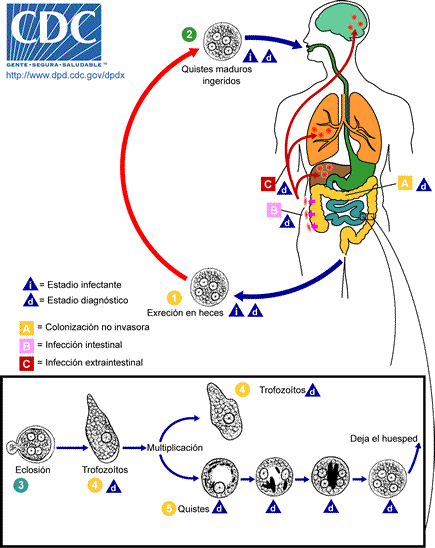
\includegraphics[width=\columnwidth]{A.imagenes/ACV-BioSan-Parasit-EHistolyticaCbios}
		\caption[Ciclo biológico de \textit{E. histolytica}.]{Ciclo biológico de \textit{E. histolytica}.\\Vehículo: agua o comida (directo no saprozoico).\\Vía: oral.\\Agente: quistes. \label{fig:PARASIT:EHistolyticaCBios}}
	\end{figure}
\end{multicols}
\subsubsection{Control}
\begin{itemize}[itemsep=0pt,parsep=0pt,topsep=0pt,partopsep=0pt]
	\item Saneamiento de aguas residuales
	\item Profilácticos.
	\item Medidas higienicas y lavado de alimentos (lejía alimentaria).
\end{itemize}
\subsubsection{Patología}
El periodo de incubación es de 2 a 21 días, el prepatente de 2 a 7 y el patente se puede extender durante años.
\begin{itemize}[itemsep=0pt,parsep=0pt,topsep=0pt,partopsep=0pt]
	\item\textbf{Disenteria\footnote{En griego: \textit{Muchas deposiciones}} amebiana} o \textbf{Amebiosis intestinal}: se produce en la fase inicial en el intestino. Los trofozoitos se adsorben en la mucosa y mediante enzimas, producen una actividad lítica del tejido, formando una úlcera <<en cuello de botella>>, reproduciendose en ella en forma de <<panal de abeja>>. Si la ulceración llega a la submucosa, pueden ir a localizaciones secundarias (enfermedad extraintestinal).
	\item\textbf{Amebomas}: granulomas en el cólon (sólo en el 1 \% de los casos, y en Latinoamérica).
	\item\textbf{Abcesos extraintestinales}: a través del torrente sanguineo, las amebas colonizan el SNC, hígado o lo hacen a través de las pleuras (con ulceraciones intestinales sangrantes).
\end{itemize}
\subsubsection{Sintomatología} 
\begin{itemize}[itemsep=0pt,parsep=0pt,topsep=0pt,partopsep=0pt]
	\item\textbf{Lesiones intestinales}: dolor abdominal; diarrea sanguinolienta , abunudante y con mucus; fiebre alta y dolor de cabeza. Si la amebiosis prospera, se pude producir paro cardiaco por agotamiento o peritonitis por perforación intestinal.
	\item\textbf{Lesiones extraintestinales}: se forman abcesos (formación con amebas externas e internas con tejido necrótico) en cerebro, bajo el nombre de meningoencefalitis amebiana secundaria; o abcesos hepáticos, en piel, pulmón y pene.
\end{itemize}
\subsubsection{Diagnosis}
\begin{itemize}[itemsep=0pt,parsep=0pt,topsep=0pt,partopsep=0pt]
	\item\textbf{Etiológico}: mediante examen de heces, distinguiendo a comensales como \textit{Entamoeba coli} o \textit{E. dispar}, esta última mediante técnicas moleculares.
	\item\textbf{Inmunodiagnóstico}: de escasa sensibilidad en caso de no haber amebas en sangre. Se hace mediante IFI, inmunohemoaglutinación, o ELISA (sensibilidad del 95 \% en casos extraintestinales, 70 \% en intestinales y 10 \% en asintomáticos; IgM dan positivo el 64 \% de las veces).
	\item\textbf{PCR}: permite descartar a \textit{E. dispar}.
\end{itemize}
\newpage
\section{Amebas anfiozoicas}
Las amebas anfizoicas\footnote{En griego: \textit{Ambas vidas} [libre y parasitaria].} siguen un ciclo biológico facultativo pudiendo vivir de forma exozoica como amebas de vida libre o endozoica como parasitos unicelulares. Su ciclo parasitario surge de una penetración accidental en el hospedador. Actualmente, se está dando un proceso de adaptación al parasitismo. Producen, por llevar acabo su acción primaria en el cerebro, una meningoencefalitis amebiana primaria que, por confusión en el diagnóstico y la falta de coevolución, resulta ser virulenta y mortal. Los géneros que afectan al ser humano son \textit{Naegleria fowleri}, \textit{Acanthamoeba cultbersoni}, \textit{Balamuthia} y \textit{Sappinia}; siendo las dos primeras las más incidentes.
\subsubsection{Morfología}
\begin{multicols}{2}
	\subsection{\textit{Naegleria fowleri}}
	Presenta tres estados. En todos los casos, el núcleo sólo es visible con microscopio de contraste de fases.
	\begin{itemize}[itemsep=0pt,parsep=0pt,topsep=0pt,partopsep=0pt]
		\item\textbf{Trofozoito ameboide}: muy activos metabolomicamente, no tienen forma constante por la emisión de pseudópodos, por los que se mueven por las superficies. Presentan un ectoplasma externo, hialino y sin orgánulos celulares; y un endoplasma interno, rugoso, con orgánulos celulares y el núcleo en posición central.
		\item\textbf{Trofozoito flagelado}: resultante del proceso a un medio líquido de las formas ameboides, o por medios poco ricos. Temporal, no presenta ectoplasma. Es ovalado, con endoplasma típico y dos flagelos polares.
		\item\textbf{Quistes}: capaces de soportar condiciones extremas, son redondeados, esféricos, con una membrana externa gruesa con perforaciones, núcleo central y endoplasma denso.
	\end{itemize}
	\columnbreak
	\subsection{\textit{Acanthamoeba cultbersoni}}
	Presenta dos estados:
	\begin{itemize}[itemsep=0pt,parsep=0pt,topsep=0pt,partopsep=0pt]
		\item\textbf{Trofozoito}: poco activo metabolicamente, sin forma constante, presenta un único núcleo y dos zonas diferenciadas: un ectoplasma externo, hialino y sin orgánulos celulares; y un endoplasma interno, rugoso, con orgánulos celulares. Tiene dos tipos de prolongaciones: filópodos, o pseudópodos espinosos, y acantopodinas, o lobópodos redondeados.
		\item\textbf{Quistes}: presenta las mismas estructuras del trofozoito (ectoplasma, endoplasma y un núcleo poco visible), carece de prolongaciones. El endoplasma tiene conformaciones poliédricas.
	\end{itemize}
\end{multicols}
\begin{figure}[H]
	\centering
	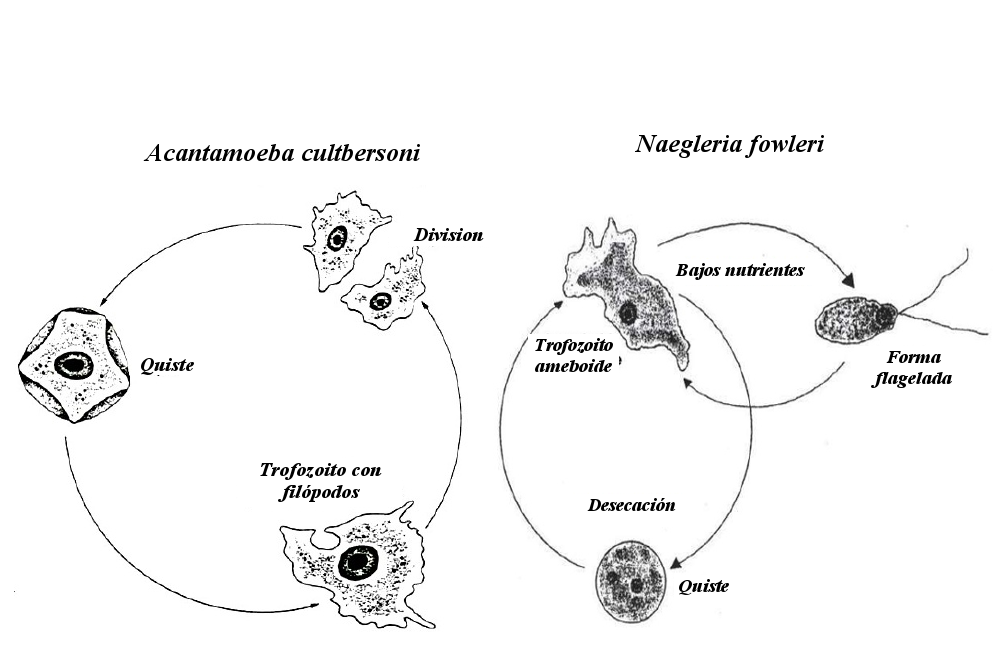
\includegraphics[trim=0 0.1cm 0.01cm 4cm,clip,width=0.55\columnwidth]{A.imagenes/ACV-BioSan-Parasit-AAnfizMorf}
	\caption[Morfología y ciclo vital \textit{N. fowleri} y \textit{A. cultbersoni}]{Morfología y ciclo vital libre de las dos amebas anfizoicas más comunes: \textit{N. fowleri} y \textit{A. cultbersoni}.\label{fig:PARASIT:AAnfizMorf}}
\end{figure}
\subsubsection{Ciclo biológico}
Estas amebas se hallan presentes en el fondo de lagos y pozas (\textit{Naegleria} es capaz de vivir en aguas a 50º C y \textit{Acanthamoeba} vive en filtros de aire con \textit{L. pneumophila}). Estas amebas, por medio de turbulencias, ascienden a la superficie. Por aerosoles, estas amebas ingresan en la cavidad nasal del hospedador, llegando a su epitelio olfativo. De éste, siguiendo sus vías axonales, viajan al lóbulo olfativo, extendiendose por el encéfalo a la par que se multiplican asexualmente. En el caso de \textit{A. cultbersoni} puede llevar consigo a \textit{L. pneumophila}. Es capaz a su vez de introducirse por heridas en la piel o por la córnea.
\subsubsection{Control}
\begin{itemize}[itemsep=0pt,parsep=0pt,topsep=0pt,partopsep=0pt]
	\item Evitar bañarse en aguas no controladas.
	\item Cloración y salinización (>0.7 \%) de aguas.
	\item Adición de poliheximida al 2 \% para líquidos de lentillas.
\end{itemize}
\begin{figure}[H]
	\centering
	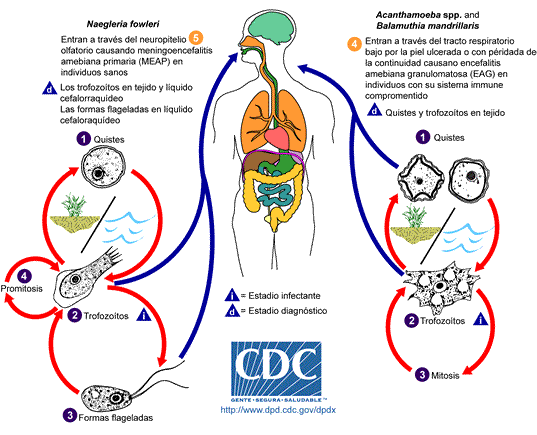
\includegraphics[width=0.65\columnwidth]{A.imagenes/ACV-BioSan-Parasit-AAnfizCbios}
	\caption[Ciclos biológicos de \textit{N. fowleri} y \textit{A. cultbersoni}.]{Ciclos biológicos de \textit{N. fowleri} y \textit{A. cultbersoni}. Vehículo: aerosoles infectados (directo no saprozoicos), Vía: nasal, parenteral u ocular, Agente: Trofozoito.\label{fig:PARASIT:AAnfizCBios}}
\end{figure}
\subsubsection{Patología}
\begin{itemize}[itemsep=0pt,parsep=0pt,topsep=0pt,partopsep=0pt]
	\item\textbf{Meningoencefalitis amebiana primaria}: su periodo de incubación es de 1 a 3 días, o raramente de 7 a 14 días. La principal acción del parásito es una acción traumática de bloqueo, generando focos necróticos en el encéfalo. La sintomatología comienza con el comienzo de las divisiones y es facilmente confundible con una meningitis bacteriana: cefaleas, fiebre alta, nauseas, vómitos, rigidez de la nuca, encefalitis, creación de zonas necróticas y de consistencia blanda, meninges purulentas y congestión del bulbo olfativo. La muerte llega, en el 95 \% de los casos, a los 4 o 6 días.
	\item En el caso de \textit{A. cultbersoni}, causa:
	\begin{itemize}[itemsep=0pt,parsep=0pt,topsep=0pt,partopsep=0pt]
		\item\textbf{Encefalitis amebiana granulomatosa}: de desarrollo lento (periodo de incubación desconocido), se produce cuando el parásito se introduce por heridas y se distribuye por sangre. Allí donde se multiplica el parásito, forma una membrana. Los síntomas: afección nerviosa en varios puntos, dolor de cabeza insidioso, fiebre esporádica, ataxia y desorientación.
		\item\textbf{Queratinitis}: se produce ante situaciones de inmunocompromiso, traumas epiteliales en la córnea y agua de limpieza de lentillas contaminada con amebas. Se produce una destrucción de la córnea por inflamación, ulceración y perforación. Sus síntomas se confunden con infecciones por infecciones por herpes o bacterias: opacidad de la córnea, iritis, irritación ocular, lagrimeo excesivo, dolores agudos y pérdida de visión.
	\end{itemize}
\end{itemize}
\subsubsection{Diagnóstico}
\subsubsection{\textit{Naegleria fowleri}}
\begin{itemize}[itemsep=0pt,parsep=0pt,topsep=0pt,partopsep=0pt]
	\item\textbf{Clinico}: buscando síntomas y antecedentes del paciente.
	\item\textbf{Etiológico}: en líquido cefalorraquidio se puede encontrar viva y movil con Giemsa y tinciones de Wright. Cultivable en agar \textit{E. coli}.
	\item\textbf{Inmunológico}: Inmunofluorescencia o inmunoperoxidasa en necropsias.
	\item\textbf{PCR}.
\end{itemize}
\subsubsection{\textit{Acanthamoeba culbertsoni}}
\begin{itemize}[itemsep=0pt,parsep=0pt,topsep=0pt,partopsep=0pt]
	\item\textbf{Etiológico}: identificada en biopsias cutáneas o cerebrales (granulomas) o mediante su cultivo a 22 y 37 C
	\item\textbf{Inmunológico}: mediante IFI o ELISA con antígenos extraidos de tejido fijados en formol.
	\item\textbf{PCR}.
\end{itemize}
\newpage
\section{Ciliados}
\subsection{\textit{Balantidium coli}}
La balantidiosis es una enfermedades transmitidas por parásitos protozoarios intestinales relativamente comunes y de amplia distribución mundial. De ciclos y sintomatología parecida \textit{Giardia lambia}, son relativamente distantes en cuanto a su taxonomía.
\subsubsection{Morfología}
\textit{Balantidium coli} es un protozoo cosmopolita ciliado (siendo el único parásito de humanos ciliado). Tiene dos formas:
\begin{itemize}[itemsep=0pt,parsep=0pt,topsep=0pt,partopsep=0pt]
	\item \textbf{Trofozoito}: mide entre 30 y 300 $\mu$m de largo y entre 25 y 120 $\mu$m de ancho. En su parte externa presenta una película de la que surgen cilios en filas longitudinales, que, en el citoplasma, se interconectan en una estructura denominada cinetodesma. Esta estructura se encarga de la organización sincrónica del movimiento, conociéndose al total de la estructura que realiza la función como infraciliatura. Presenta dos núcleos, un macronúcleo (grande, de forma de J o judía, relacionada con funciones tróficas) y un micronúcleo (pequeño, situado en la concavidad del macronúcleo, relacionado con funciones de reproducción). Tiene en el citoplasma dos vacuolas contráctiles. Así mismo, es relevante una estructura, el citostoma. Esta estructura es una invaginación en forma de embudo no ciliada de este protozoo por la que introduce el alimento. Se compone de una abertura externa (peristoma), que se continúa con un conducto (citofaringe) que acaba en un ciego junto a la vacuola alimentaria. En el polo contrario se halla el citopigio, por donde se exocitan los desechos.
	\item \textbf{Quiste}: de un tamaño de entre 45 y 75 $\mu$m de diámetro, son estructuras esféricas recubiertas de una pared resistente. Tras esa pared se descubre una célula muy similar al trofozoito: sin citostoma, ciliada y con los dos núcleos.
\end{itemize}
\begin{multicols}{2}
	\begin{figure}[H]
		\centering
		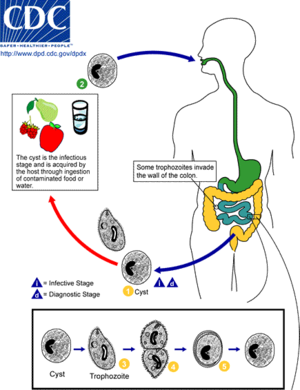
\includegraphics[width=\columnwidth]{A.imagenes/ACV-BioSan-Parasit-BcoliCBios}
		\caption[Ciclo biológico de \textit{B. coli}]{Ciclo biológicos de \textit{B. coli}. Vehículo: comida y agua infectadas, Vía: oral, Agente: Quiste.\label{fig:PARASIT:BColiCBios}}
	\end{figure}
	\columnbreak
	\vspace*{5.4cm}
	\begin{figure}[H]
		\centering
		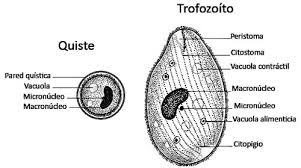
\includegraphics[width=\columnwidth]{A.imagenes/ACV-BioSan-Parasit-BcoliMorf}
		\caption[Morfología de \textit{B. coli}]{Morfología de \textit{B. coli}. A la izquierda, el quiste con sus secciones; a la derecha, la forma parasitaria intestinal.\label{fig:PARASIT:BColiMorf}}
	\end{figure}
\end{multicols}
\subsubsection{Ciclo biológico}
La localización de \textit{B. coli} es, principalmente, el intestino grueso (ciego y colon) de cerdo, chimpancés, ratas y humanos. Tiene un ciclo directo, siendo monoxeno. Este parásito entra por vía oral, vehiculizado en agua o alimentos contaminados con quistes de esta especie. En el intestino delgado acontece la desenquistamiento. En el intestino, las formas de trofozoito se alimentan de enterocitos del hospedador, bacterias, mucus y eritrocitos (balantidiosis extraintestinal). Estos protozoos poseen un metabolismo anaerobio. En el intestino se reproducen por fisión binaria transversal (homeotetogónica), o, cuando hay cepas diferentes, mediante conjugación.
\subsubsection{Epidemiología y control}
Su distribución es cosmopolita, siendo más frecuente en zonas tropicales y subtropicales. Suele aparecer como brote epidémico, siendo su prevalencia del 1 al 53\%. Es más incidente en zonas con gran cabaña porcina. La población de riesgo es aquella gente en contacto con excrementos de animales (jardineros, población de granjas,…) así como de lugares de higiene deficiente y gran concentración de población (psiquiátricos, cárceles,…)

Los sistemas de control comienzan con una adecuada educación sanitaria, unida a ciertas medidas higiénicas, control de aguas y sistemas adecuados de saneamiento de letrinas.
\subsubsection{Patogenia y sintomatología}
La infección por \textit{Balantidium coli} provoca infecciones desde asintomáticas a graves. Así, puede ser una infección de tipo agudo o crónico. Se trata de un invasor secundario, es decir, sólo es capaz de infectar en conjugación con factores concomitantes: estrés, malnutrición, dietas ricas en glúcidos y pobre en proteínas, presencia de otros microorganismos que irriten las mucosas, aclorhidria o alcoholismo.

Los síntomas que provoca son semejantes a \textit{Entamoeba histolytica}, formación de úlceras (planas y redondas), diarreas (en casos graves, con sangre y mucus), nauseas, vómitos, cólicos intestinales y, relacionado con estos, deshidratación e insuficiencia renal. En casos de malnutrición, la muerte puede sobrevenir a los 3 ó 5 días. A pesar de que hay cepas poseedoras de hialuronidasa, si no existe lesión previa, no invade tejidos extraintestinales. En caso de que la haya, se dan casos de peritonitis e invasión de pulmón e hígado. Así mismo, existen también casos asintomáticos crónicos (portadores sanos).
\subsubsection{Diagnóstico}
El diagnóstico de la balantidiasis se hace mediante diagnóstico etiológico por coprología, identificándose trofozoitos en casos de disentería y quistes en casos crónicos.
\newpage
\section{Flagelados: \textit{Trypanosomatide}}
La familia \textit{Trypanosomatide}, género \textit{Trypanosoma}, tiene importancia en el campo de la Parasitología por causar dos enfermedades: la enfermedad del sueño y el Mal de Chagas. Este género se divide en dos subgéneros o secciones, que son:
\begin{itemize}[itemsep=0pt,parsep=0pt,topsep=0pt,partopsep=0pt]
	\item \textbf{Subgénero \textit{Trypanozoon}} o \textbf{Sección salivaria}: transmitidos por la picadura de un vector, la mosca tsé-tsé (género \textit{Gossina}), son los que producen la enfermedad del sueño. Son los tripanosomas africanos: \textit{Trypanosoma Trypanozoon brucei gambiense} (produce la enfermedad del sueño de África Central y Occidental) y \textit{Trypanosoma Trypanozoon brucei rhodesiense} (enfermedad del sueño de África Oriental). 
	\item \textbf{Subgénero \textit{Schizotrypanum}} o \textbf{Sección \textit{Stercoraria}}: transmitidos por contaminación con heces infectadas del vector, producen el Mal de Chagas. Son los tripanosomas americanos: \textit{Trypanosoma cruzi}.
\end{itemize}

La enfermedad del sueño se creyó controlada en la década de los 50, pero sufrió un repunte en 1970. Actualmente, se estiman 20000 casos reales, con una población en riesgo de 70 millones de personas. Las zonas donde se dan los tripanosomas africanos es el África tropical. \textit{T. gambiense}, productora del 98\% de los casos se da al oeste del Rift Valley, mientras que \textit{T. rhodesiense} se da al oeste del Rift Valley. Existen regiones sobre esta cordillera montañosa, como Uganda, donde coexisten las dos especies.
\newpage
\subsection{\textit{Trypanosoma brucei}}
\subsubsection{Morfología}
\textit{Tripanosoma brucei} es una especie parásita heteroxena (tiene dos hospedadores, uno invertebrado (género \textit{Gossina}, la mosca tsé-tsé), y uno cordado). Una característica común en todos los tripanosomas es que son flagelados, ya sea libre o en un bolsillo flagelar, todas las fases tienen flagelo. Así mismo, todas las formas del parásito tienen un único núcleo, un aparato de Golgi, un retículo endoplásmico y una mitocondria, que en su interior guarda un kinetoplasto (reserva de DNA), siempre cercano al kinetosoma (lugar de donde surge el flagelo), y una serie de microtúbulos subpediculares. Las formas posibles son:
\begin{itemize}[itemsep=0pt,parsep=0pt,topsep=0pt,partopsep=0pt]
	\item \textbf{Promastigote}: de forma alargada, presentan una estructura, el quinetosoma, cerca del quinetoplasto, donde nace el flagelo.
	\item \textbf{Epimastigote}: similar al promastigote, presenta una pequeña membrana ondulante antes de quedar libre.
	\item \textbf{Tripomastigote}: presenta una membrana ondulante por todo el cuerpo y una mitocondria desarrollada.
	\item \textbf{Esferomastigote}: esféricos, presentan un pequeño flagelo que se pega a la superficie.
	\item \textbf{Paramastigote}: esféricos, con un flagelo corto y libre.
\end{itemize}

Los tripanosomas se caracterizan por dos características, el polimorfismo (distintas formas de un mismo parásito en un mismo hospedador por distintas etapas de desarrollo) y el pleomorfismo (distintas variaciones en la morfología de una forma parasitaria en un mismo hospedador) (ver figura \ref{fig:PARASIT:TBruceiMorfA}). Estas características forman parte de estrategias de enmascaramiento antigénico. Así, las formas polimórficas son:
\begin{itemize}[itemsep=0pt,parsep=0pt,topsep=0pt,partopsep=0pt]
	\item Formas tripomastigote intestinales en el hospedador invertebrado.
	\item Formas epimastigote en el hospedador invertebrado.
	\item Formas tripomastigote metacíclicas en el hospedador invertebrado.
	\item Formas tripomastigote sanguíneas en el hospedador vertebrado.
	\item Formas amastigote y epimastigote en el hospedador vertebrado (en chancro tripanosómico).
\end{itemize}
El pleomorfismo se da en las formas tripomastigote sanguíneas en el hospedador cordado son:
\begin{itemize}[itemsep=0pt,parsep=0pt,topsep=0pt,partopsep=0pt]
	\item \textbf{Formas largas}: mitocondrias sencilla con crestas cortas tubulares. Precisan grandes cantidades de oxígeno y glucosa. Muy activas, son abundantes en sangre y linfa.
	\item \textbf{Formas intermedias}: más evolucionadas, con mitocondrias con crestas alargadas.
	\item \textbf{Formas cortas}: redondeadas, cortas con un flagelo de 1 $\mu$m. Mitocondrias muy elaboradas con gran actividad metabólica. Son las formas infectantes para la mosca.
\end{itemize}
\begin{figure}[H]
	\centering
	\subfigure[Distintas formas de \textit{T. brucei} dentro de los hospedadores.\label{fig:PARASIT:TBruceiMorfA}]{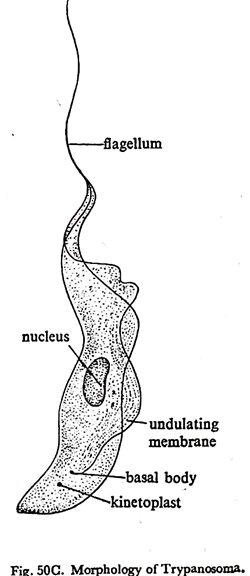
\includegraphics[width=0.5\columnwidth]{A.imagenes/ACV-BioSan-Parasit-TbruceiMorf2}}
	\subfigure[Morfología del tripomastigote.]{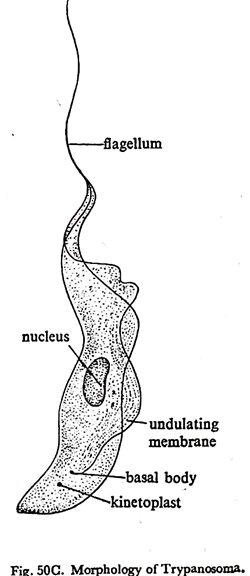
\includegraphics[trim=0 1cm 0 0,scale=0.55,clip]{A.imagenes/ACV-BioSan-Parasit-TbruceiMorf2}}
	\caption[Morfología de \textit{T. brucei}]{Distintas formas parasitarias y ciclo de la morfología de \textit{T. brucei} y detalle de la constitución del tipomastigote sanguineo.\label{fig:PARASIT:TBruceiMorf}}
\end{figure}
\subsubsection{Ciclo biológico}
El ciclo biológico del parásito comienza cuando una mosca tse-tsé sana pica a un animal infectado, con tripomastigotes en sangre. Estos ingresan en el  tracto digestivo de la mosca, dándose una multiplicación por fisión binaria longitudinal. Cuando se verifica, se obtienen, ya en la zona media del intestino, tripomastigotes intestinales. Estos atraviesan la membrana peritrópica, por el espacio endoperitrópico, buscando las glándulas salivales de la mosca. En ellas se da una multiplicación, saliendo, por fisión binaria, dos epimastigotes de cada tripomastigote. Tras ello, ocurre otra multiplicación, formándose tripomastigotes metacíclicos, la forma infectiva para el hospedador vertebrado. Así, cuando la mosca se alimenta de otro hospedador vertebrado, con la saliva viajan los tripomastigotes metacíclicos.

En la picadura, el parásito tiene dos posibilidades: a) pasa directamente a sangre en forma de tripomastigote; o b) se da una multiplicación en los tejidos anejos a la picadura de forma masiva, transformándose en epimastigotes y generándose por ello el chancro tripanosómico. Dentro de ese chancro tripanosómico se encuentran formas esferomastigote y amastigote. Estas se transforman en tripomastigote y pasan a sangre, llegando a otros órganos y multiplicándose en ellos. Cuando una mosca sana chupa la sangre a este hospedador, se lleva tripomastigotes que le infectan, reiniciándose el ciclo.

El tiempo de desarrollo en la mosca es de 3 semanas, mientras que el ser humano es de entre 5 y 12 días, sirviendo de portador. En el tripomastigote metacíclico se forman gran variedad de antígenos, preparándose para ser infectantes. Esta es una forma de evitar que el sistema inmune emita una respuesta que elimine el parásito (gran variabilidad antigénica que evite una respuesta inmune eficaz). Además, el parásito ha creado distintas maneras para perdurar en el tiempo. En el hospedador vertebrado, se dan dos formas de tripomastigote en sangre: las cortas y las largas. Las formas cortas son las infectantes para la mosca y se dan en  momentos en los que baja el número por una respuesta inmune eficaz, asegurándose que pasa a la otra fase del ciclo. Las formas largas se dan cuando hay gran cantidad de estos parásitos.
\begin{figure}[H]
	\centering
	%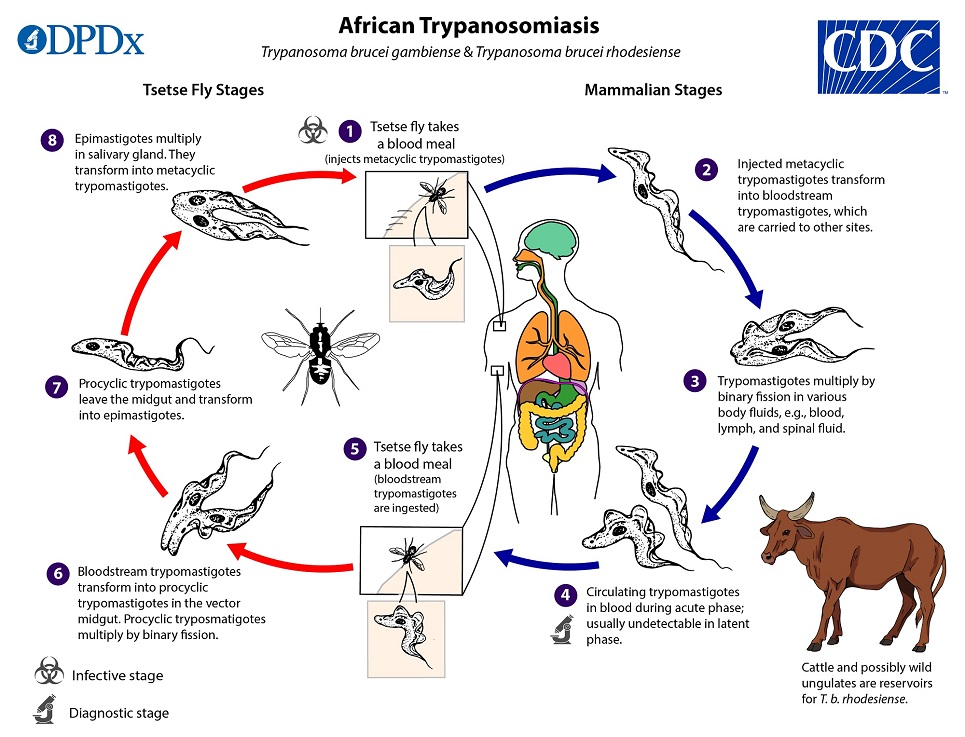
\includegraphics[width=0.8\columnwidth]{A.imagenes/ACV-BioSan-Parasit-TbruceiCBios}
	\caption[Ciclo vital de \textit{T. brucei}]{Ciclo vital de \textit{T. brucei}. Vector: mosca del género \textit{Gossina}. Vía: parenteral. Agente: tripomastigote metacíclico.\label{fig:PARASIT:TBruceiCBios}}
\end{figure}
\subsubsection{Transmisión y control}
Las principales formas de transmisión del parásito son las picaduras del vector (la mosca tsé-tsé) y transfusiones de sangre y trasplantes de órganos. Así, los principales puntos de control son el control del vector mediante insecticidas, repelentes y mosquiteras; diagnóstico y tratamiento de los infectados (control de los reservorios) y control en las transfusiones de sangre y trasplantes de órganos.
\subsubsection{Patología}
De las especies que pueden provocar la enfermedad del sueño, ambas dos provocan la enfermedad con una duración distinta: \textit{T gambiense} cursa de forma crónica (varios meses o años), y \textit{T rhodesiense} cursa de forma aguda (unas semanas a 9 meses). En ambos es común el tiempo de incubación (de 1 a 21 días se puede hallar en sangre), el periodo prepatente (de 7 a 21 días) y el periodo patente (de meses a años). Así mismo, también es común la sintomatología de la enfermedad, que se divide en tres periodos:
\begin{enumerate}[itemsep=0pt,parsep=0pt,topsep=0pt,partopsep=0pt]
	\item \textbf{Periodo inicial} (o de <<incubación>>): dura entre 6 a 14 días, hasta que el parásito llega a sangre. En este periodo se distinguen dos fases:
	\begin{itemize}[itemsep=0pt,parsep=0pt,topsep=0pt,partopsep=0pt]
		\item De 2 a 3 días tras la infección, se forma, en el lugar de la picadura, el chancro tripanosómico: un edema localizado, de centro vesiculoso, bordes descamados y doloroso al tacto. En ese chancro se dan las primeras multiplicaciones del parásito.
		\item De 5 a 12 días tras la infección, se da la parasitemia (elevada si es T rhodesiense) con una fiebre alternante semanal (provocada por picos de parásitos en sangre, hasta que se activa la respuesta inmune, se acompaña de síntomas inespecíficos (periodo prodrómico: malestar general, dolor de cabeza y articulaciones,…)) y anemia normocrónica (por la adsorción de antígenos solubles a eritrocitos sanos, produciendo su lisis por: eritrofagocitosis, activación del complemento o producción de una hemolisina)
	\end{itemize}
	\item \textbf{Periodo segundo}: se pueden encontrar parásitos en linfa, lo que genera una inflamación de los ganglios (sobre todo cervicales) conocidos como signo de Winterbottom, tras 7 a 12 días de la infección. Tras varias multiplicaciones en los ganglios, se da una adenopatía generalizada. En este periodo el parásito llega a distintos órganos: corazón (cardiomegalia, pancarditis), pulmón (edema, congestión por fallo cardiaco).
	\item \textbf{Tercer periodo}: se da la llegada al cerebro del parásito, afectando gravemente al SNC: cefalea intensa, rigidez del cuello, apatía, falta de interés por el trabajo, insomnio, somnolencia, cambio de personalidad, desintegración de funciones del SNC, convulsiones, ataxia, meningitis, y muerte por coma, insuficiencia cardiaca o neumonía.
\end{enumerate}
\subsubsection{Diagnóstico}
\begin{itemize}[itemsep=0pt,parsep=0pt,topsep=0pt,partopsep=0pt]
	\item \textbf{Diagnóstico clínico}: basado en la presencia del chancro tripanosómico, el signo de Winterbottom y fiebre alternante semanal.
	\item \textbf{Diagnóstico etiológico}: búsqueda de tripanosomas en:
	\begin{itemize}[itemsep=0pt,parsep=0pt,topsep=0pt,partopsep=0pt]
		\item \textbf{Chancro}: se hallan formas amastigote y esferomastigote.
		\item \textbf{Sangre}: se hallan tripomastigotes excepto a los 12 días posteriores a la infección; 2 ó 3 días posteriores a la parasitemia y al final de la enfermedad.
		\item \textbf{Linfa}: se encuentran tripomastigotes.
	\end{itemize}
	\item \textbf{Diagnóstico serológico o indirecto}: mediante HAI, ELISA, IFI o F.C.
\end{itemize}
\newpage
\subsection{\textit{Trypanosoma cruzi}}
La enfermedad de Chagas, enfermedad así llamada por el descubridor de su agente etiológico, Carlos Chagas, está causada por el protozoo flagelado \textit{Trypanosoma cruzi}. Descrito en 1909, y llamado así por Oswaldo Cruz, no fue hasta 1930 cuando se le relacionó directamente con el mal de Chagas.

Su distribución se asocia con la de su vector, la vinchuca, chinche asesina o chinche besucona. Esta es la parte continental del mar Caribe, costa pacífica de Méjico, Ecuador, Bolivia, norte y centro de Chile y Argentina y costa atlántica de Brasil (a excepción de la desembocadura del Amazonas). De 120 millones de personas expuestas, entre 16 y 18 millones están parasitadas. Por el mal de Chagas hay unas 50000 muertes anuales en estas zonas, siendo el responsable de la muerte del 30\% de los adultos en Brasil. En Argentina parasita a 3 millones de personas; en EEUU, a 300000; y en España, hasta a unos 68000.
\subsubsection{Morfología}
\begin{multicols}{2}
	\textit{Trypanosoma cruzi} presenta polimorfismo y pleomorfismo. En cuanto a su polimorfismo, se dan varias fases tanto en el hospedador invertebrado como en el cordado, siendo:
	\begin{itemize}[itemsep=0pt,parsep=0pt,topsep=0pt,partopsep=0pt]
		\item \textbf{Hospedador invertebrado}: según avanza en su intestino se dan formas esferomastigote (tracto digestivo inicial), epimastigote (intestino medio) y tripomastigote metacíclico (final del intestino). 
		\item \textbf{Hospedador vertebrado}: en él se dan las formas de amastigote (chagoma), tripomastigote (en sangre) y formas intracelulares intermedias (en células parasitadas, amastigotes).
	\end{itemize}
	\columnbreak
	\begin{figure}[H]
		\centering
		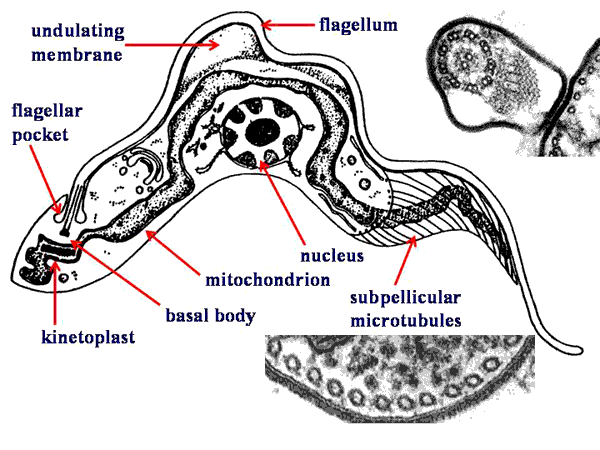
\includegraphics[width=0.8\columnwidth]{A.imagenes/ACV-BioSan-Parasit-TcruziMorf2}
		\caption[Morfología de \textit{T. cruzi}]{Morfología de \textit{T. cruzi}, tripomastigote en sangre. Detalles de los microtúbulos del flagelo. \label{fig:PARASIT:TCruziMorf}}
	\end{figure}
\end{multicols}

Con respecto a formas pleomórficas, se dan las siguientes:
\begin{itemize}[itemsep=0pt,parsep=0pt,topsep=0pt,partopsep=0pt]
	\item En las formas de \textbf{tripomastigote} (sangre del hospedador vertebrado), existen tres formas: cortas, intermedias y largas. Son formas más flexuosas que otros tripanosomas.
	\item En la fase de \textbf{epimastigote} en el intestino medio del vector, existen dos formas: medias y largas.
\end{itemize}
\subsubsection{Ciclo biológico}
\textit{T. cruzi} tiene un ciclo vital que se desarrolla entre dos hospedadores: la vinchuca, un artrópodo de la familia \textit{Reduvidae}, subfamilia \textit{Triatominae}, perteneciente a los géneros: \textit{Triatoma}, \textit{Pastrongylus}, \textit{Rhodnius}; y un mamífero: armadillo, roedores, marsupiales, perros, gatos, humanos,\dots en ninguno de los do hay reproducción sexual, solo se dan multiplicaciones por fisión binaria.

El ciclo comienza con la picadura de una vinchuca parasitada durante la noche (atraída por el CO$_2$ que expele su víctima), normalmente cerca del ojo o los labios. Tras ello, defeca, dejando junto a la herida heces con tripomastigotes metacíclicos. Al rascarse, se introducen en la herida, o cualquier otro punto de entrada (córnea, mucosas,\dots) dándose allí la primera multiplicación. En la piel, cambian de forma al introducirse en las células, transformándose en amastigotes. Una vez se han dado muchas fisiones binarias, el pseudoquiste estalla y libera los amastigotes, que cambian de forma a tripomastigotes en sangre. Estos viajan por el organismo, infectando a otras células (preferentemente a la musculatura no voluntaria). Una vez contactan con una célula, cambian su forma a amastigote, multiplicándose en su interior. Repetirán el ciclo indefinidamente.

El mecanismo de entrada de los tripomastigotes en la célula es sencillo. El parásito se deja fagocitar por la célula objetivo, quedando incluido en una vacuola parasitaria. La célula, mediante la fusión con enzimas líticos, trata de eliminarlo, pero el parásito segrega una enzima, la Tc-Tox, que rompe esas vacuolas, pudiendo darse la multiplicación.

El ciclo biológico termina cuando el hospedador vertebrado es picado de nuevo por una chinche sana, llevándose con la sangre las formas tripomastigote. Estos avanzan por el tracto digestivo y, en el estómago, se transforman en epimastigote, tras lo cual se multiplican, y siguen viajando hasta el fin el intestino del vector, donde se multiplican y se transforman en tripomastigotes metaciclicos, que saldrán de nuevo por las heces.

El tiempo de desarrollo en el vertebrado es de entre 4 a 5 semanas hasta encontrar formas infectantes. En la vinchuca, es de 10 a 8 días.
\begin{figure}[H]
	\centering
	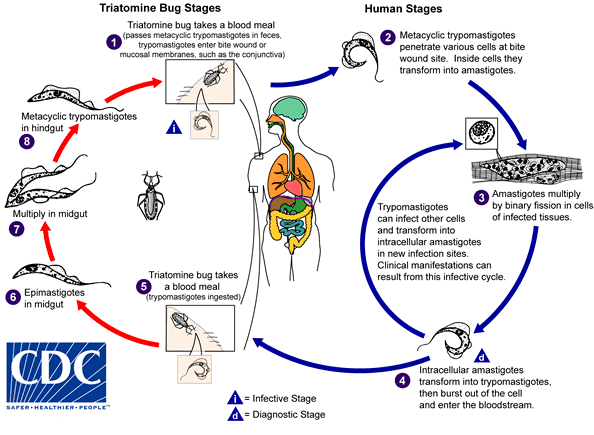
\includegraphics[width=0.7\columnwidth]{A.imagenes/ACV-BioSan-Parasit-TcruziCBios}
	\caption[Ciclo vital de \textit{T. cruzi}]{Ciclo vital de \textit{T. cruzi}. Vector: artŕopodo de la subfamilia \textit{Triatominae}. Vía: parenteral. Agente: tripomastigote metacíclico.\label{fig:PARASIT:TCruziCBios}}
\end{figure}
\subsubsection{Transmisión y control}
Los modos de transmisión más comunes son:
\begin{enumerate}[itemsep=0pt,parsep=0pt,topsep=0pt,partopsep=0pt]
	\item Contaminación de mucosas o heridas por heces de un vector que contengan tripomastigotes metacíclicos.
	\item Transfusiones de sangre y trasplantes de órganos.
	\item Transplacentaria o durante la lactancia
	\item Material quirúrgico o de tatuador contaminado con heces de este parásito.
	\item Contaminación por ingesta de alimentos contaminados con heces contaminadas con tripomastigotes.
\end{enumerate}
Así, las medidas de control son:
\begin{enumerate}[itemsep=0pt,parsep=0pt,topsep=0pt,partopsep=0pt] 
	\item Evitar la picadura de la chinche. Para ello, se invierte en educación sanitaria y en eliminar a la vinchuca del ambiente doméstico y peridoméstico, mediante fumigación, pinturas con insecticidas, barreras físicas (mosquiteras) y alejando a reservorios (otros animales) de ese entorno.
	\item Control en sangre y órganos de la presencia del parásito.
	\item Diagnóstico en embarazos.
	\item Esterilización de material contaminado.
	\item Higiene alimentaria.
\end{enumerate}

La existencia de reservorios mantiene el problema, por ello se hace tan importante el asilar a animales susceptibles de ser reservorios del entorno peridoméstico.
\subsubsection{Patogenia}
La tripanosomosis americana, la enfermedad de Chagas o el mal silenciosos es una enfermedad causada por T. cruzi. Este parásito lleva, sobre todo, una acción traumática de destrucción de las células (cuando una célula del hospedador se infecta, se le denomina pseudoquiste) por masiva multiplicación del parásito en su interior.

El periodo de incubación de la enfermedad es de unos 5 a 20 días, siendo el periodo prepatente de 1 a 2 meses; y el periodo patente de hasta 20 años.

En cuanto a la sintomatología del mal de Chagas, se distinguen cuatro etapas:
\begin{enumerate}[itemsep=0pt,parsep=0pt,topsep=0pt,partopsep=0pt] 
	\item \textbf{Fase inicial} (o de incubación): se puede observar el chagoma (zona enrojecida, eritematosa, de tacto duro y doloroso junto al lugar de la picadura del parásito); linfadenitits (inflamación de los ganglios cercanos al lugar de la infección) y el signo de Romaña (edema de párpado y conjuntiva).
	\item \textbf{Fase aguda}: se da la aparición de la parasitemia y la diseminación de a otros tejidos 60 días después a la infección, apareciendo por ello fiebre alta, dolores musculares o inespecíficos, malestar general (por la multiplicación del parásito en el medio intracelular). Aparecen lesiones en distintos órganos: hepatomegalia, cardiomegalia, miocarditis (provoca taquicardias que, si no son tratadas, llevan a la muerte) y daños en el SNC (aneurismas, irritabilidad y embotellamiento mental (en niños, puede producir un coma que puede llevar a la muerte))
	\item \textbf{Fase latente}: en esta fase, asintomática, el parásito continúa multiplicándose en el interior de las células, pero no genera signos ni síntomas.
	\item \textbf{Fase crónica}: aparece a los 10 o 20 años de la infección. Afecta a ganglios del sistema parasimpático en esófago y colon (10\% de los casos), y provoca distensiones de esófago y colon (megaesófago (regurgitación) y megacolon (estreñimiento), respectivamente) irreversibles.
\end{enumerate}
\subsubsection{Diagnosis}
\begin{itemize}[itemsep=0pt,parsep=0pt,topsep=0pt,partopsep=0pt] 
	\item \textbf{Diagnóstico clínico}: basado en el chagoma y el signo de Romaña.
	\item \textbf{Diagnóstico etiológico}: se puede realizar en:
	\begin{itemize}[itemsep=0pt,parsep=0pt,topsep=0pt,partopsep=0pt] 
		\item Recogida de muestras en el chagoma (macrófagos o histocitos con amastigotes en su interior)
		\item En ganglios inflamados cercanos al lugar de la infección (con tripomastigotes en su interior)
		\item En periodos de fiebre, se hallan tripomastigotes en sangre.
		\item \textbf{Cultivo} de muestras en medio NNN (en caso de poco número, para aumentar su concentración).
		\item \textbf{Xenodiagnóstico}: dejar picar a una chinche sana a un individuo sospechoso y, tras esperar entre 10 y 30 días, buscar en su intestino las diversas formas del parásito.
	\end{itemize}
	\item \textbf{Diagnóstico indirecto}: mediante IFI, ELISA y PCR (reacciones cruzadas con \textit{Leishmania}). Análisis de proteínas por espectrometría (proteómica, 99\% de especificidad).
\end{itemize}
\newpage
\section{Otros Flagelados}
\subsection{\textit{Leishmania} spp}
La leishmaniosis está causada por distintas especies del género \textit{Leishmania}, que se transmite por medio de un vector, un mosquito del género \textit{Phlebotomus} (Viejo Mundo, también conocido como <<beatilla>>) o \textit{Lutzomyia} (Nuevo Mundo), causando hasta tres tipos de parasitosis: leishmaniosis cutánea, mucocutánea y visceral o kala-azar. Las especies son:
\begin{itemize}[itemsep=0pt,parsep=0pt,topsep=0pt,partopsep=0pt] 
	\item Especies responsables de la \textbf{Leishmaniosis visceral}, transmisor \textit{Phlebotomus}:
	\begin{itemize}[itemsep=0pt,parsep=0pt,topsep=0pt,partopsep=0pt] 
		\item[$ $]	\textit{L. (L.) donovani}
		\item[$ $] \textit{L. (L.) infantum} (en España)
		\item[$ $] \textit{L. (L.) archivaldi}
		\item[$ $] \textit{L. (L.) chagasi} (en América, transmisor \textit{Lutzomyia})
	\end{itemize}
	\item Especies responsables de \textbf{Leishmaniosis cutáneas}:
	\vspace*{-0.5cm}
	\begin{multicols}{2}
		\subitem En el Viejo Mundo\footnote{conocido como \textit{Botón de Oriente}}, transmisor \textit{Phlebotomus}.
		\begin{itemize}[itemsep=0pt,parsep=0pt,topsep=0pt,partopsep=0pt]
			\item[$ $] \textit{L. (L.) tropica}
			\item[$ $] \textit{L. (L.) major}
			\item[$ $] \textit{L. (L.) aethiopica} (cutánea difusa)
			\item[$ $] \textit{L. (L.) infantum} (en España)
		\end{itemize}
		\columnbreak
		\subitem En el Nuevo Mundo: transmisor \textit{Lutzomyia}
		\begin{itemize}[itemsep=0pt,parsep=0pt,topsep=0pt,partopsep=0pt]
			\item[$ $] \textit{L. (L.) mexicana}
			\item[$ $] \textit{L. (L.) amazonensis}
			\item[$ $] \textit{L (L.) enrietti}
			\item[$ $] \textit{L. (L.) venezuelensis}
			\item[$ $] \textit{L. (L.) pifanoi}
		\end{itemize}
	\end{multicols}
	\vspace*{-0.5cm}
	\item Especies responsables de \textbf{Leishmaniosis mucocutánea} (Nuevo Mundo) \textit{Lutzomyia}
	\begin{itemize}[itemsep=0pt,parsep=0pt,topsep=0pt,partopsep=0pt]
		\item[$ $] \textit{L. (V.) braziliensis} (espundia)
		\item[$ $] \textit{L. (V.) guyanensis} (pianbois)
		\item[$ $] \textit{L. (V.) panamensis} (afección nasofaríngea rara)
		\item[$ $] \textit{L (LV) peruviana} (uta)
	\end{itemize}
\end{itemize}

En cuanto a su epidemiología:
\begin{itemize}[itemsep=0pt,parsep=0pt,topsep=0pt,partopsep=0pt] 
	\item \textbf{Prevalencia mundial}: 12 millones parasitados (350 millones expuestos) principalmente en regiones tropicales y subtropicales.
	\item \textbf{Incidencia mundial}: 500.000 nuevos casos al año
	\item \textbf{Incidencia en España}: 100-120 casos anuales.
	\item \textbf{Enfermedad reemergente} en Europa: Brotes en países meridionales de Europa (700 casos autóctonos)
\end{itemize}
\subsubsection{Morfología}
Leishmania pertenece a la familia \textit{Trypanosomatide} teniendo también pleomorfismo y polimorfismo:
\begin{itemize}[itemsep=0pt,parsep=0pt,topsep=0pt,partopsep=0pt] 
	\item \textbf{Polimorfismo}: se da por las diferentes formas presentes en su ciclo vital en los dos hospedadores: amastigote (vertebrados) y promastigote, amastigote, esferomastigote y paramastigote (invertebrados)
	\item \textbf{Pleomorfismo}: sólo se da en formas promastigote del estómago del mosquito, habiendo formas neptomonadidas (más de 12 $\mu$m) y haptomonadidas (menos de 12 $\mu$m).
\end{itemize}

Así mismo, el género \textit{Leishmania} se divide en dos subgéneros, según donde se desarrolle en el aparato digestivo del mosquito:
\begin{itemize}[itemsep=0pt,parsep=0pt,topsep=0pt,partopsep=0pt] 
	\item \textbf{Sección \textit{Suprapylaria}}: son especies del subgénero \textit{Leishmania}. El parasito sólo se desarrolla en la región anterior y media del intestino del vector.
	\item \textbf{Sección \textit{Peripylaria}}: son especies del subgénero \textit{Viannia}. Se desarrolla en la zona anterior, media y posterior del parásito.
\end{itemize}

Independientemente del subgénero y especie, la fase infectante para el vertebrado es la de promastigote, y para el mosquito, la de amastigote.
\begin{figure}[htpb]
	\centering
	\subfigure[Fases y morfología en el hospedador vertebrado y en el vector de las dos formas de \textit{Leishmania} spp. \textbf{N}: Núcleo; \textbf{K}: kinetoplasto; \textbf{F}: Flagelo]{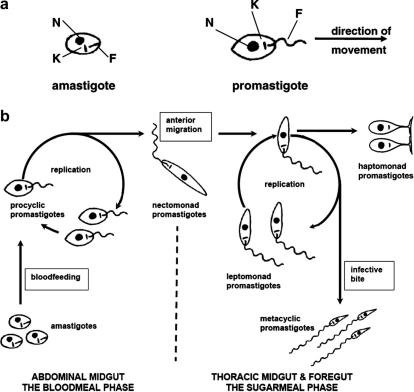
\includegraphics[width=0.475\columnwidth]{A.imagenes/ACV-BioSan-Parasit-LeishmaniaMorf1}}
	\subfigure[Morfología de \textit{Leishmania} (concretamente \textit{L. donovani}) de su vista al microscopio electrónico del tripomastigote en vertebrados]{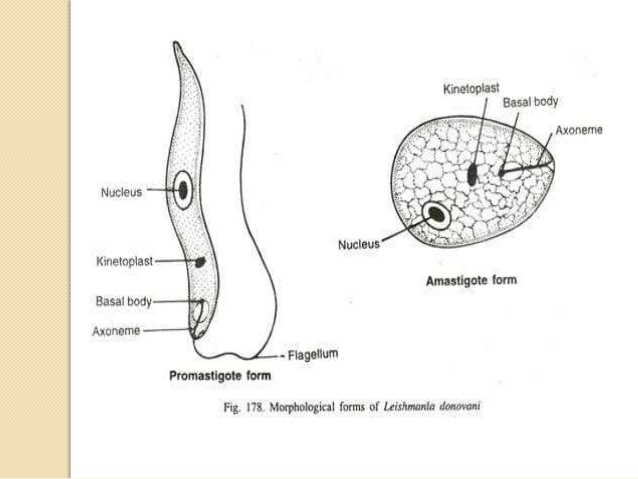
\includegraphics[trim=3cm 3cm 0 0,clip,width=0.475\columnwidth]{A.imagenes/ACV-BioSan-Parasit-LeishmaniaMorf2}}
	\caption[Morfología de \textit{Leishmania}]{Morfología de \textit{Leishmania}, con descripción de sus partes visibles y de sus ciclos biológicos. \label{fig:PARASIT:LeishmaniaMorf}}
\end{figure}
\subsubsection{Ciclo biológico}
Se trata de un parásito heteroxeno (dos hospedadores: vertebrados (roedores, cánidos, carnívoros, caballos y humanos); e invertebrados (mosquitos)). Existen dos ciclos: el zoonótico, en el que es necesario el mosquito; y el antroponótico, consistente en la transmisión entre seres humanos, bien por mosquitos, bien por jeringuillas. 

El ciclo zoonotico comienza cuando un mosquito infectado pica a un individuo no infectado. En el momento de la picadura, con su saliva, el mosquito inyecta formas promastigote que son fagocitadas por los macrófagos. Sobreviven a las vesículas líticas de los macrófagos gracias a la liberación de la proteasa gp63 que protege de la degradación lisosomal, así como de su cubierta polisacarídica (lipofosfoglicano, LPG). Tras penetrar en la célula, se transforman en amastigotes (en el momento de la secreción de gp63) y comienzan a multiplicarse.
 
Tras muchas multiplicaciones, el macrófago estalla, liberando amastigotes que serán de nuevo fagocitados, continuando la parasitosis. El ciclo continúa con la picadura por parte de un mosquito sano que tras la ingesta, los amastigotes, en su estómago, se multiplican y cambian de conformación a promastigote (formas neptomonadidas en su zona media del estómago y, en la banda estomodal, formas haptomonadidas). En el esófago, se transforman en paramastigotes que al avanzar a la faringe pasan a formas promastigote. En especies de la sección peripilaria también se da multiplicación en el píloro, siendo el resto del ciclo de la misma forma.
\begin{figure}[H]
	\centering
	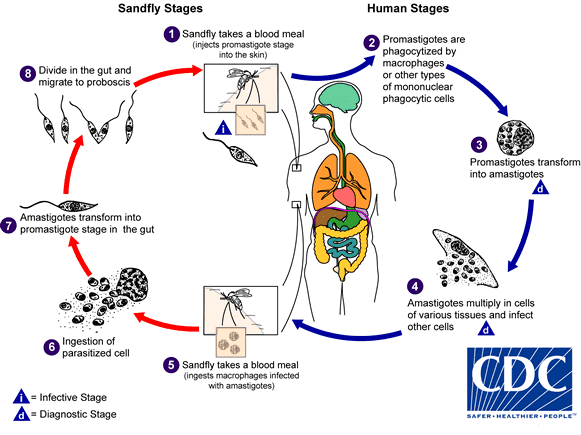
\includegraphics[width=0.75\columnwidth]{A.imagenes/ACV-BioSan-Parasit-LeishmaniaCBios}
	\caption[Ciclo biológico de \textit{Leishmania} spp]{Ciclo biológico de \textit{Leishmania} spp. Vector: mosquito; Agente: promastigote; Vía: parenteral.}
\end{figure}
\subsubsection{Control}
\begin{itemize}[itemsep=0pt,parsep=0pt,topsep=0pt,partopsep=0pt] 
	\item Evitar la picadura del insecto mediante mosquiteras, repelentes,$\dots$
	\item Control de reservorios y control y tratamiento de los infectados.
	\item No compartir jeringuillas (resulta especialmente incidente en pacientes seropositivos contagiados por el uso compartido de jeringuillas, siendo además oportunista (gran desarrollo de la enfermedad en pacientes con linfocitos CD4$^+$ en niveles menores a 50 udd/mL)).
\end{itemize}
\subsubsection{Vector y epidemiologia}
La leishmaniosis se transmite por la inoculación en la picadura de formas promastigote presentes en la saliva de dos mosquitos: \textit{Phlebotomus} y \textit{Lutzomyia}. Estos mosquitos son capaces de sobrevivir 1 mes infectados, siendo transmisores a partir de los 3 o 4 días de la infección. Pican las hembras al atardecer, yendo a zonas oscuras, haciendo vuelos cortos y rastreros en días sin viento. Tienen piezas bucales cortas, pudiendo picar solo en zonas de piel desnuda. Los reservorios de la enfermedad son carnívoros y mamíferos medianos.

Estos mosquitos se diferencian por:
\begin{table}[H]
	\centering
	\begin{tabular}{cc}
		\rowcolor{black}\textcolor{white}{\textit{\textbf{Phlebotomus}}}&\textcolor{white}{\textit{\textbf{Lutzomyia}}}\\
		Propios del Viejo Mundo&Propios del Nuevo Mundo\\
		(Mediterráneo, Próximo Oriente, India, África Tropical)&Zonas tropicales.\\
		\rowcolor{hiperlightgray}Regiones semiáridas (grietas, huecos en árboles, suelo)&Zonas boscosas (selva)\\
		Necesitan humedad pero no corrientes de agua&Precisan de un alto grado de humedad\\
		\hline
	\end{tabular}
	\caption{Comparativa entre los diferente vectores de \textit{Leishmania}.}
\end{table}
\subsubsection{Patología y sintomatología}
Se diferencian tres tipos de leishmaniosis, causadas por las citadas especies del género \textit{Leishmania}.
\paragraph{Cutánea}
Es la única de las leishmaniosis que es capaz de producir una cierta inmunidad. Su periodo de incubación es muy variable: de días a años. En el punto de la picadura del mosquito, el punto de la infección, se forma una pápula roja que, a los pocos días, se forma una costra y, tras ella, se ulcera (la parasitosis puede complicarse debido a otras infecciones secundarias que aprovechen la úlcera para introducirse en el organismo). La úlcera se cierra, se da la curación espontánea, siendo así efectiva la gran respuesta inmune, en un plazo de dos meses a un año, dejando una cicatriz despigmentada.

Esta enfermedad la provocan dos especies distintas, \textit{L. tropica} y \textit{L. major}, con dos comportamientos ciertamente distintos:
\begin{table}[H]
	\centering
	\begin{tabular}{cc}
		\rowcolor{black}\textcolor{white}{\textit{\textbf{Leishmania tropica}}}&\textcolor{white}{\textit{\textbf{Leishmania major}}}\\
		Se da en zonas urbanas muy pobladas. Sin reservorios.&Zonas rurales poco habitadas.\\
		&Con reservorios (animales domésticos).\\
		\rowcolor{hiperlightgray}Pápula seca, roja y con muchos amastigotes en ella.&Pápula húmeda, roja, bulbosa y con pocos\\
		\rowcolor{hiperlightgray} Persiste meses sin ulcerar.& amastigotes en ella. Se ulcera con facilidad.\\
		Su curación sólo da inmunidad frente a \textit{L. tropica}.&Produce inmunidad frente a\textit{ L. tropica} y \textit{L. major}\\
		\hline
	\end{tabular}
	\caption{Leishmaniosis cutánea: principales agentes y comparación}
\end{table}

Otro tipo de leishmaniosis cutáneas son:
\begin{itemize}[itemsep=0pt,parsep=0pt,topsep=0pt,partopsep=0pt]
	\item \textbf{Leishmaniosis cutánea difusa}: provocada por \textit{L. aethiopica} y \textit{L. pifani}. Se trata de una leishmaniosis parecida a la cutánea en la que las úlceras se difunden por todo el tegumento.
	\item\textbf{Úlcera del chiclero}: causada por \textit{L. mexicana}. El mosquito (genero \textit{Lutzomyia}) que vive en el árbol del chicle (en sus hojas y en la corteza) pica sobre todo en la oreja, donde degrada la piel y el cartílago de zonas anexas a la picadura.
\end{itemize}
\paragraph{Mucocutánea}
La especie tipo de esta parasitosis es \textit{Leishmania Viannia braziliensis}. El 90\% de los casos de esta enfermedad se hallan entre Bolivia, Brasil y Perú. La picadura del mosquito da lugar a una lesión en la piel parecida a la de la leishmaniosis cutánea: formación de una pápula roja a la que siguen lesiones secundarias por infección de ésta. Cuando se cura, comienzan a verse daños en mucosas de otras partes del cuerpo: se forman pápulas que acaban por ulcerarse y son especialmente predispuestas a infectarse, generando infecciones secundarias que acaban por llevar a la muerte si no hay tratamiento. La formación de úlceras se relaciona con metástasis en tabique nasal y faringe, pudiendo además destruir partes blandas de nariz, paladar o labios.
\paragraph{Visceral o Kala-azar}
Esta leishmaniosis es muy prevalente en la zona de la India y África. El periodo de incubación de esta enfermedad es muy variable (de 10 días a un año). Primeramente aparece una lesión cutánea que pasa desapercibida (pequeña pápula) y donde se da la primera multiplicación. A partir de ahí, pasa a sangre, llegando a hígado y bazo, donde se multiplicará en el interior de los macrófagos de estos órganos.
La multiplicación del parásito se asocia a una disminución de células sanguíneas (anemia normocítica, leucopenia y trombocitopenia) lo que genera una hiperplasia de hígado y bazo en su función de más elementos formes sanguíneos (hepatomegalia, esplenomegalia) y un incremento inespecífico de las inmunoglobulinas y un descenso de la albúmina.

La sintomatología de la enfermedad se desarrolla de la siguiente forma: aparece una fiebre inicial, vómitos y un agotamiento progresivo. Pueden aparecer pigmentaciones oscuras en la piel, lo que se ha llamado fiebre negra. Se produce una distensión abdominal y aparecen dolores en el abdomen acompañados, al final de la enfermedad, de disenterías. Sin tratamiento provoca la muerte en 2 ó 3 años. Las manifestaciones más agudas cursan con fiebre, frío, vómitos, edemas, hemorragias en las mucosas, dificultad respiratoria y muerte entre los 6 y 12 meses posteriores a la infección. 
\subsubsection{Diagnóstico}
\begin{itemize}[itemsep=0pt,parsep=0pt,topsep=0pt,partopsep=0pt] 
	\item \textbf{Mucocutánea y cutánea}
	\begin{itemize}[itemsep=0pt,parsep=0pt,topsep=0pt,partopsep=0pt] 
		\item \textbf{Clínico}: se puede identificar inequívocamente por las lesiones generadas en la piel.
		\item \textbf{Etiológico}: se puede optar mediante el visionado directo de muestras de piel de pápulas (se observan macrófagos con Leishmania en su interior), o, si no hay gran cantidad de parásitos, concentrarlo mediante cultivo en NNN o RPMI y agar sangre. También existe la posibilidad del xenodiagnóstico, ya sea por inoculación a un mosquito sano y su posterior disección, o inoculándosela a un ratón.
		\item \textbf{Inmunodiagnóstico}: pueden hacerse pruebas inmunohistoquímicas que identifiquen  al parasito dentro de las células; ELISA, IFI o Western Blot, aunque existen reacciones cruzadas con \textit{Trypanosoma} spp, \textit{Mycobacterium leprae} y \textit{Mycobacterium tuberculosis}; y por último, la intradermorreacción de Montenegro (inyección de antígenos de Leishmania y ver si existe un eritema (positivo si es mayor de 5 mm.). La prueba tiene una sensibilidad del 95\%, pero una vez hecha, provoca una inmunidad en el paciente que genera falsos positivos al repetirla.
		\item \textbf{PCR}: resulta especialmente útil para identificar la especie causante.
	\end{itemize}
	\item \textbf{Visceral}: Dado que la pápula no es llamativa y los otros síntomas pueden llevar a confusión, no existe diagnóstico clínico.
	\begin{itemize}[itemsep=0pt,parsep=0pt,topsep=0pt,partopsep=0pt] 
		\item \textbf{Etiológico}: Leishmania no se puede encontrar en frotis sanguíneos, recurriéndose a punciones de médula ósea, hepática y bazo. Estas muestras recogidas se pueden concentrar mediante cultivo en RPMI o NNN; o se puede realizar xenodiagnóstico (inocularle el aislado a animales de experimentación). 
		\item \textbf{Indirecto}: Se puede hacer mediante IFI o ELISA. No tiene valor la prueba de Intradermorreacción de Montenegro. 
		Otra prueba específica para el kala-azar o leishmaniosis visceral es la reacción de formol-leuco-gelificación, que permite detectar la gran elevación de anticuerpos asociados a esta enfermedad. El mecanismo es el siguiente: se toman unas 20 gotas de suero problema al que se le
	\end{itemize} añaden 2 gotas de formol al 40\%. Se espera 30 minutos y se observa: si se gelifica, la reacción es positiva; si permanece líquido, la reacción es negativa.
\end{itemize}
\newpage
\subsection{\textit{Giardia lambia}}
La giardiosis es una enfermedades transmitidas por parásitos protozoarios intestinales relativamente comunes y de amplia distribución mundial. De ciclos y sintomatología parecida \textit{Balantidium coli}, son relativamente distantes en cuanto a su taxonomía.
\subsubsection{Morfología}
\textit{Giardia lamblia} es un flagelado anaerobio intestinal de distribución cosmopolita, pero de mayor incidencia en zonas cálidas y templadas. Carece de mitocondrias y aparato de Golgi, se reproducen por fisión binaria longitudinal. Posee dos formas:
\begin{itemize}[itemsep=0pt,parsep=0pt,topsep=0pt,partopsep=0pt]
	\item \textbf{Trofozoito}: con dos núcleos, piriformes (en forma de careta, siendo los núcleos los ojos), posee simetría longitudinal. Tiene 4 pares de flagelos a cada lado: un par anterolateral, un par ventral, un par posterolateral y un par caudal. Estos últimos nacen en la parte anterior (en la parte redondeada), recorriendo el axonema todo el citoplasma, rígidos, formando el funis. Los núcleos se sitúan a ambos lados del funis, teniendo grandes nucléolos. Presentan también dos cuerpos medios curvos. En su citoplasma hay gran cantidad de ribosomas, RE y gránulos de glucógeno. La parte redondeada recibe el nombre de disco suctor, estructura con la que se adhiere a las vellosidades intestinales.
	\item \textbf{Quiste}: son ovalados, con 2 (inmaduros) o 4 (maduros) núcleos. Tiene restos de axonemas y de los cuerpos medios. Presentan un citoplasma muy colapsado.
\end{itemize}
\subsubsection{Ciclo biológico}
Se trata de un ciclo biológico directo monoxeno, teniendo varios reservorios (perros, gatos, ganado, primates). Una vez entran los quistes de Giardia lamblia en el organismo (por vía oral, vehiculizado por alimentos o agua contaminados por quistes (de 2 o 4 núcleos (inmaduros y maduros, respectivamente)). Al llegar al duodeno, eclosionan, obteniéndose 1 ó 2 trofozoitos, que continúan dividiéndose a lo largo que viajan por el intestino. Al llegar al colon, la falta de humedad hace que comience la fase de enquistación, que, ya sean maduros o inmaduros, salen al exterior por las heces, siendo capaces de poder reiniciar el ciclo.

Las moscas pueden actuar como transmisiones mecánicos de los quistes.
\begin{multicols}{2}
	\begin{figure}[H]
		\centering
		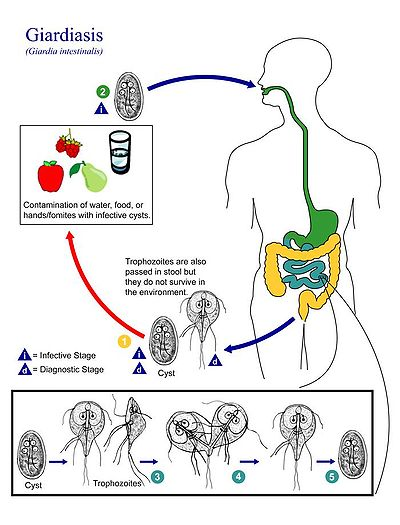
\includegraphics[width=0.895\columnwidth]{A.imagenes/ACV-BioSan-Parasit-GlambiaCBios}
		\caption[Ciclo biológico de \textit{G. lambia}]{Ciclo biológicos de \textit{G. lambia}. Vehículo: comida y agua infectadas, Vía: oral, Agente: Quiste.\label{fig:PARASIT:GLambiaCBios}}
	\end{figure}
	\columnbreak
	\begin{figure}[H]
		\centering
		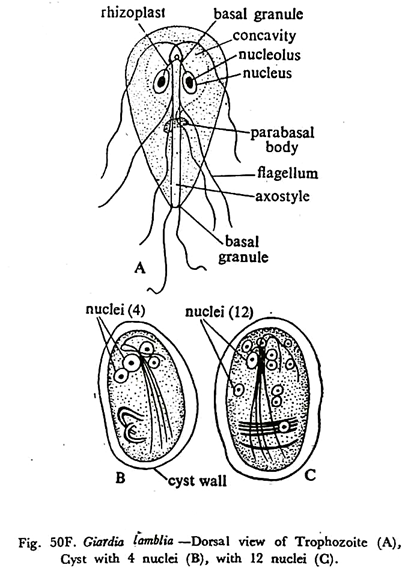
\includegraphics[trim= 0 1cm 0 0,clip,width=0.9\columnwidth]{A.imagenes/ACV-BioSan-Parasit-GlambiaMorf}
		\caption[Morfología de \textit{G. lambia}]{Morfología de \textit{G. lambia}. En la parte superior (\textbf{A}), la forma parasitaria; en la parte inferior, la forma de resistencia e infecciosa, el quiste, con (\textbf{B}) 4 núcleos y con (\textbf{C}) 8 núcleos.\label{fig:PARASIT:GLambiaMorf}}
	\end{figure}
\end{multicols}
\subsubsection{Epidemiología}
Presenta prevalencias variables (un 2\% en adultos y un 7\% de niños en países desarrollados, frente a un 33\% en países en desarrollo). Es la infección protozoaria más común en el ser humano, con una prevalencia de 280 millones de personas, y una incidencia de 500000 casos anuales (600 en España). La dosis infectiva es de entre 10 y 100 quistes, pero un individuo parasitado llega a arrojar hasta 10 billones de estas formas de manera diaria. La principal población de riesgo son los niños, personal de guarderías, turistas, ganaderos y homosexuales (contacto oral-anal).

Las principales medidas de control son el lavado adecuado de alimentos (3 gotas de Na(ClO) por litro de agua, durante 10 minutos) y de manos, para evitar la transmisión. Así mismo, el control de aguas, la correcta manipulación de alimentos y la higiene personal y comunitaria.
\subsubsection{Patogenia y sintomatología}
\textit{Giardia lamblia} tiene un tiempo de incubación de entre 7 y 20 días, un periodo patente desde horas hasta un par de días, y un periodo patente de meses o años. No presentan acción patógena traumática (no invaden las mucosas), siendo su acción patógena la deformación (aplanamiento) de las vellosidades intestinales.

Esta acción genera irritación en el intestino, que causa casi todos los síntomas de la enfermedad: nauseas, vómitos, dolor epigástrico sordo o vago, meteorismo, irritación duodenal por exceso de producción de mucus, síndrome de malabsorción (no se absorben las grasas ni vitaminas liposolubles, generando adelgazamiento y pérdida de apetito; y en el caso de niños, retraso mental) fiebre y diarrea (que pueden ser crónicas o agudas (continuas o intermitentes) con esteatorrea (heces grasientas). En algunas ocasiones se puede ver afectada la vesícula biliar (provocando ictericia y cólicos biliares) por acción mecánica obstructiva (impiden el paso de la bilis).
\subsubsection{Diagnosis}
\begin{itemize}[itemsep=0pt,parsep=0pt,topsep=0pt,partopsep=0pt]
	\item \textbf{Clínico}: un síntoma indicativo, pero no excluyente, de giardiosis es la esteatorrea (heces grasientas)
	\item \textbf{Etiológico}: se puede hacer mediante coprología (recogida de heces de tres días distintos y se examinan directamente o mediante técnicas de concentración (Bailenger) y posterior visualización), recogida de muestras por aspirado duodenal (y posterior visualización) o mediante PCR (aplicado a las muestras, permitiendo reconocer subtipos). 
	\item \textbf{Inmunológico}: se basa en la búsqueda y detección de coproantígenos en muestras de heces mediante ELISA, IFD.
\end{itemize}
\newpage
\subsection{\textit{Trichomonas vaginalis}}
De las dos especies del género \textit{Trichomona} que pueden vivir en el cuerpo humano, la única que presenta una importancia clínica es \textit{T. vaginalis}. La otra, \textit{T. hominis}, es un parasito comensal del intestino.

\textit{Trichomonas vaginalis} parasita la vagina y las glándulas prostáticas. Cosmopolita, su incidencia mundial es de 180 millones de casos (200 en España) cada año. La población de riesgo son prostitutas y el 100\% de las compañeras sexuales de varones tricomoniósicos. 
\subsubsection{Morfología}
\textit{Trichomonas vaginalis} no forma quistes. El trofozoito emite pseudópodos y está flagelado. Presenta 4 flagelos libres y uno unido a la membrana plasmática que la curva (recurrente), formando una membrana ondulante. Este último flagelo no sale, frente a T. hominis, que si es libre.

Presenta un núcleo, aparato de Golgi,  y una fibra solo visible al MET, denominada pelta que forma parte de las fibras parabasales. Así mismo, tiene un citostoma solo visible al MET y una gran cantidad de formaciones rígidas con función de soporte. Estas últimas son el axostilo (estructura que viaja desde el polo anterior al posterior, saliendo de la célula) y la costa (estructura cilíndrica y delgada situada bajo la membrana ondulante que la soporta y permite dar la forma). Junto a estas estructuras se encuentran gran cantidad de hidrogenosomas, paracostales y paraaxostilares, según se encuentren al lado de que estructura.

Esta célula se alimenta sobre todo de bacterias de la vagina.
\subsubsection{Ciclo biológico}
El ciclo de \textit{Trichomonas vaginalis} es un ciclo directo y sin reservorios (se dan infecciones de persona a persona). Transmitido por vía venérea, en el parto a recién nacidas y por instrumental ginecológico mal esterilizado. 

Las medidas de control más eficientes son el uso de preservativos y la detección y tratamiento adecuado de hospedadores (sobre todo varones asintomáticos).
\begin{multicols}{2}
	\begin{figure}[H]
		\centering
		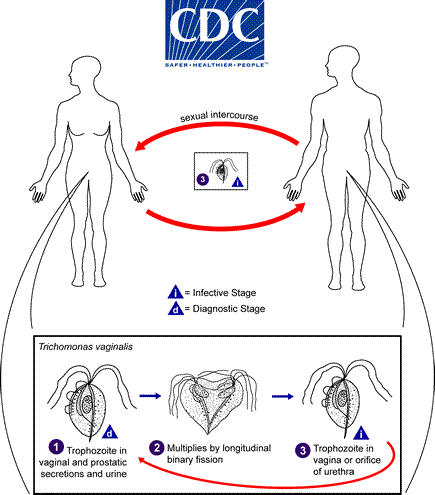
\includegraphics[width=\columnwidth]{A.imagenes/ACV-BioSan-Parasit-TVaginalisCBios}
		\caption[Ciclo biológico de \textit{T. vaginalis}]{Ciclo biológicos de \textit{T. vaginalis}. Vehículo: infección directa, Vía: sexual, Agente: Trofozoito.\label{fig:PARASIT:TvaginalisCBios}}
	\end{figure}
	\columnbreak
	\begin{figure}[H]
		\centering
		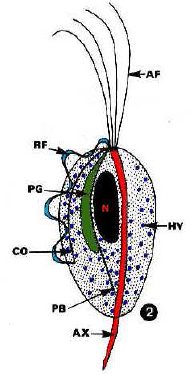
\includegraphics[width=0.585\columnwidth]{A.imagenes/ACV-BioSan-Parasit-TVaginalisMorf}
		\caption[Morfología de \textit{T. vaginalis}]{Morfología de \textit{T. vaginalis}. \textbf{AF}: Flagelos libres; \textbf{RF}: Membrana ondulante (flagelo); \textbf{PG}: Pelta o aparato de Golgi; \textbf{CO}: costa; \textbf{N}: núcleo; \textbf{HY}: citoplasma (hidrogenosomas); \textbf{PB}: fibras parabasales; \textbf{AX}: axostilo.\label{fig:PARASIT:TvaginalisMorf}}
	\end{figure}
\end{multicols}
\subsubsection{Patogenia y sintomatología}
La trichomonosis tiene un periodo de incubación de 4 a 28 días, un periodo prepatente de 4 a 28 días, y un periodo patente de meses o años. La principal acción de Trichomonas vaginalis es una acción traumática en el cérvix, provocando inflamación. Esta inflamación provoca la degeneración del epitelio del cuello de útero, evolucionando la enfermedad de dos maneras distintas:
\begin{itemize}[itemsep=0pt,parsep=0pt,topsep=0pt,partopsep=0pt]
	\item \textbf{Agudo}: se produce un flujo vaginal lechoso, purulento y fétido, siendo prueba patente de la enfermedad.
	\item \textbf{Crónico}: el flujo vaginal no presenta tantos leucocitos como en el curso agudo, pero se halla presente \textit{T. vaginalis} y una gran cantidad de células epiteliales.
\end{itemize}

La erosión del cérvix genera predisposiciones a sufrir carcinoma y es factor de riesgo para la infección de VIH y HVS-2. En varones suele ser asintomática, generando, a veces, prostatitis, uretritis, irritación temporal en el pene, ligero ardor tras orinar o eyacular y, en contados casos, esterilidad (reversible).

La sintomatología solo se presenta en el 30\% de los individuos parasitados. Esta es: escozor, prurito vulvar y vaginal, cambio de aspecto de las secreciones vaginales, vulvitis, dolor en la parte baja del vientre, cistitis y disuria.
\subsubsection{Diagnóstico}
\begin{itemize}[itemsep=0pt,parsep=0pt,topsep=0pt,partopsep=0pt]
	\item \textbf{Etiológico}: observación directa en secreciones vaginales o prostáticas y en sedimentos urinarios (hay que tomar medidas frente a contaminación con heces (falsos positivos por \textit{Trichomonas hominis}), cultivo de muestras en medios con suero y caseína hidrolizada (durante 7 días), o mediante PCR.
	\item \textbf{Indirecto}: mediante aplicaciones de HAI, IFI o ELISA de suero del paciente. Puede cuantificarse la cantidad de parásitos.
\end{itemize}
\newpage
\section{\textit{Apicomplexa}}
Los coccidios son una clado dentro del phylum \textit{Apicomplexa}, concretamente, dentro de la clase \textit{Sporozoea}, subclase \textit{coccidia}. Este clado se caracteriza por poseer todas las características tipo del filum. Esta es la posesión del complejo apical.

El complejo apical está formado por un orificio localizado en un polo de la célula, denominado anillo polar (pudiendo haber  uno o dos), que le corresponde uno en el otro extremo (anillo posterior). Bajo este anillo polar se encuentra el conoide, una formación cónica en espiral en cuyo centro se hallan las rotrias (cuyo número varía según la especie) en cuyo final, y a lo largo del conoide se hallan los micronemas, cuerpos vesiculares con sustancias proteicas en su interior que, en el caso de protozoos intracelulares, poseen sustancias líticas que permiten parasitar a la célula diana. Surgiendo del anillo polar, y cubriendo todo el cuerpo, se hallan los microtúbulos subpediculares. Bajo la estructura citoesquelética del complejo se halla una vacuola vestigial, el apicoplasto.

Así mismo, dentro del filum se dan las siguientes formas de reproducción:
\begin{itemize}[itemsep=0pt,parsep=0pt,topsep=0pt,partopsep=0pt]
	\item \textbf{Fisión binaria} (bipartición): la más frecuente, a partir de una célula madre se forman dos células hijas por previa cariocinesis seguida de una citocinesis. Según el plano de división son: a) anárquicas (amebas, sin plano de división definido); b) longitudinal o simetrogónica (flagelados, sigue una simetría longitudinal); y c) transversal u homotetogónica (ciliados).
	\item \textbf{Esquizogonia asexual}: en este proceso, el núcleo se divide varias veces, formando un ser multinucleado (esquizonte). Cada uno de esos núcleos se rodea de una porción de citoplasma, ocurriendo la división del citoplasma. A cada célula hija se le denomina merozoito.
	\item \textbf{Esporogonia}: se trata de una fisión múltiple tras una reproducción sexual (unión de gametos. Tras la formación del zigoto, se produce una meiosis y luego repetidas meiosis. Así, del ooquiste (con el cigoto en su interior), se forma, por meiosis, dos esporoblastos que, tras una mitosis, forma dos esporoquistes, con sendos dos o más esporozoitos en su interior.
	\item \textbf{Singamia} o \textbf{reproducción sexual}: proceso de unión de gametos y fusión de núcleos para formar, en el caso de los protozoos, un cigoto diplonte. Puede ser: isogamica (los gametos son iguales) o anisogámica (gametos distintos). El primer paso, en ambos casos, es la gamogonia o gametogénesis (proceso de formación de los gametos), llevado a cabo por los gamontes (células sexuales inmaduras que originan los gametos). En el caso de la anisogamia se diferencian dos gametocitos: el microgametocito (formado por un microgamonte que se divide muchas veces formando gametos pequeños) y el macrogamtocito (generado a partir de un único macrogamonte).
	\item \textbf{Endopoligenia} y \textbf{endodiogenia}: se trata de divisiones asexuales múltiples y binarias donde se obtienen taquizoitos o bradizoitos, respectivamente. Se diferencian de la esquizogonia en que en este proceso la membrana se forma de novo y no se verifica la división hasta que están perfectamente formadas, produciéndose entonces la rotura de la membrana de la célula madre.
\end{itemize}
\newpage
\subsection{\textit{Cryptosporidium parvum}}
\subsubsection{Morfología}
\textit{Cryptosporidium parvum} es un parásito intestinal de muchos animales y, entre ellos, del ser humano. Protozoo no flagelado, es cosmopolita y eurixeno. La incidencia en España es de unos 100 a 200 casos anuales. Está considerada una enfermedad emergente (se creía que solo afectaba a ratones, pero casos de inmunodepresión permitieron su localización en humanos) y ocupacional (es frecuente en personas en contacto directo con excretas animales). La población más expuesta a esta enfermedad son los individuos inmunosuprimidos, dado que las diarreas que causa en ellos no son autolimitantes, complicándose la enfermedad. Presenta dos formas:
\begin{itemize}[itemsep=0pt,parsep=0pt,topsep=0pt,partopsep=0pt]
	\item \textbf{Trofozoito}: tiene forma alargada y pequeña, midiendo hasta 5 $\mu$m, con puntas romas en sus extremos. En su polo apical presenta el complejo apical propio del phylum \textit{Apicomplexa}. Bajo este se halla un pequeño citostoma (microporo). Presenta un núcleo grande con un nucléolo grande. En su citoplasma se halla un aparato de Golgi, un retículo endoplásmico y mitocondrias. Las formas de trofozoito reciben un nombre distinto según se originen de esporogonias, gamogonias,… su localización habitual es el interior del enterocito, entrando en el mediante fagocitosis inducida, disponiéndose bajo el borde en cepillo.
	\item \textbf{Ooquiste}: fase de resistencia, presenta una cubierta externa quística protectora, con un orificio taponado (micropilo), los esporoquistes y una masa de restos de las divisiones celulares, el residuo ooquistico. Una vez maduro, ese micrópilo se abre y deja salir las fases al exterior. En el interior de estos se forman los esporoquistes, unas estructuras cubiertas por una membrana con los esporozoitos en su interior (con su forma de coccidio típica) y un residuo esporoquistico. Forman 4 esporozoitos en su interior, en un solo esporoquiste
\end{itemize}
\subsubsection{Ciclo biológico}
La vía de infección de \textit{Cryptosporidium parvum} es la ingesta de agua o alimentos contaminados con ooquistes maduros. 

Los ooquistes aguantan el pH estomacal, abriéndose en el intestino. Los esporozoitos que surgen del ooquistes se pegan al epitelio intestinal, fijándose, redondeándose y provocando su endocitosis y formación de una vacuola que les engloba en el interior del enterocito. En el interior de la vacuola, por esquizogonia, comienza a multiplicarse, surgiendo hasta merozoitos por esquizonte. Cuando estos merozoitos crecen, hacen estallar a la célula, reiniciando el ciclo infectivo estos merozoitos. Tras varias esquizogonias, se da una gamogonia, siendo anisogámica: en la invasión de los enterocitos, parte de los merozoitos formaran microgametocitos (16 por merozoito) y parte formaran macrogametocitos (1 por merozoito). Los gametocitos se liberan y, si se encuentran, ocurre la fecundación, generando un cigoto que formará un ooquiste, pudiendo seguir dos caminos:
\begin{enumerate}[itemsep=0pt,parsep=0pt,topsep=0pt,partopsep=0pt]
	\item El ooquiste inmaduro se libera al exterior del organismo, ocurriendo ahí su maduración, formando 4 esporozoitos con un residuo ooquistico.
	\item Se da una esporogonia en el interior del hospedador, madurando en el enterocito donde se dio la fecundación, rompiendo la célula y liberándose al exterior.
	\item En personas con problemas de inmunosupresión se da el fenómeno de la endoautoinvasión: antes de ser evacuados, el ooquiste se rompe y reinicia el ciclo esquizogónico.
\end{enumerate}

Así, el principal elemento de control de esta parasitosis es el evitar ingerir ooquistes contaminados (higiene alimentaria) y el control de las excretas.
\subsubsection{Patogenia y sintomatología}
El periodo de incubación de la cryptosporidiosis es de 3 a 12 días, el periodo prepatente es de unos 4 días, siendo el patente de 2 a 4 semanas (en inmunocompetentes, llegando a ser mortal en inmunosuprimidos (endoautoinvasión)).

La acción patógena de este parásito es, principalmente, traumática en células intestinales (provoca la destrucción del epitelio intestinal). La sintomatología de esta enfermedad es, sobre todo, diarreas intensas y acuosas. En inmunosuprimidos, estos protozoos llegan a otras localizaciones extraintestinales: vesícula biliar (colecistitis y colangitis, ictericia), conductos pancreáticos (pancreatitis) o vías respiratorias (tos, ronquera).
\subsubsection{Diagnóstico}
\begin{itemize}[itemsep=0pt,parsep=0pt,topsep=0pt,partopsep=0pt]
	\item \textbf{Etiológico}: mediante coprología, tomando una muestra de heces sospechosas y, una vez aplicada una tinción Ziehl-Nielsen, buscar ooquistes (tinción verde). No se ha de confundir con restos de descamación intestinal ni con otros coccidios intestinales (Cyclospora, Cystoisospora).
	\item \textbf{Técnicas indirectas}: pueden diagnosticarse mediante técnicas de detección de ooquistes en heces por IFI o ELISA.
\end{itemize}
\begin{multicols}{2}
	\begin{figure}[H]
		\centering
		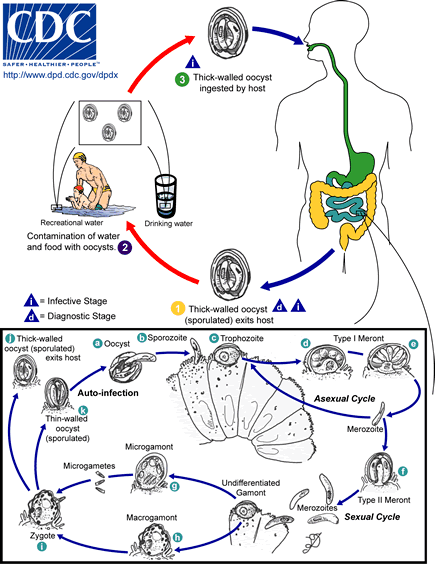
\includegraphics[width=\columnwidth]{A.imagenes/ACV-BioSan-Parasit-CparvumCbios}
		\caption[Ciclo biológico de \textit{C. parvum}]{Ciclo biológicos de \textit{C. parvum}. Vehículo: agua o alimentos contaminados, Vía: oral, Agente: Ooquiste.\label{fig:PARASIT:CparvumCBios}}
	\end{figure}
	\columnbreak
	\vspace*{2.47cm}
	\begin{figure}[H]
		\centering
		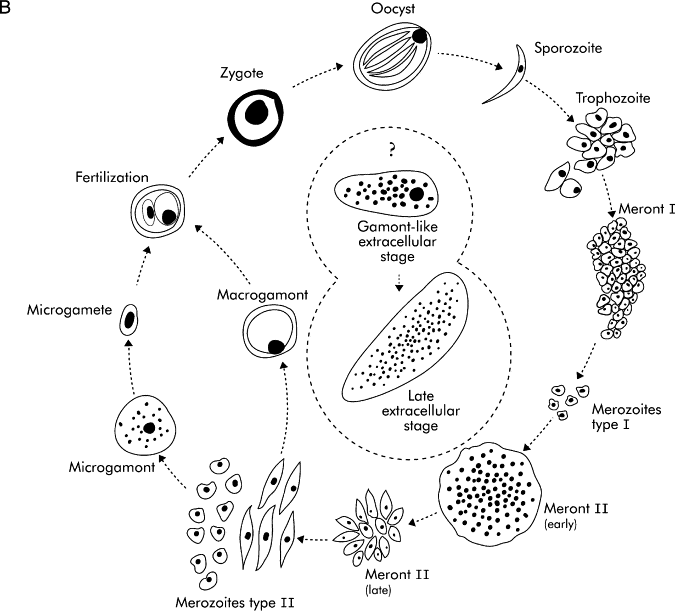
\includegraphics[width=\columnwidth]{A.imagenes/ACV-BioSan-Parasit-CparvumMorf}
		\caption[Morfología de \textit{C. parvum}]{Morfología de \textit{C. parvum} y los distintos estadíos del parásito.\label{fig:PARASIT:CparvumMorf}}
	\end{figure}
\end{multicols}
\newpage
\subsection{\textit{Cystoisospora belli}}
\subsubsection{Morfología}
Enfermedad emergente parasitaria, de distribución cosmopolita y frecuente en zonas tropicales y templadas. 
\begin{itemize}[itemsep=0pt,parsep=0pt,topsep=0pt,partopsep=0pt]
	\item \textbf{Trofozoito}: tiene forma alargada, con puntas romas en sus extremos. En su polo apical presenta el complejo apical propio del phylum \textit{Apicomplexa}. Bajo este se halla un pequeño citostoma (microporo). Presenta un núcleo grande con un nucléolo grande. En su citoplasma se halla un aparato de Golgi, un retículo endoplásmico y mitocondrias. Las formas de trofozoito reciben un nombre distinto según se originen de esporogonias, gamogonias,… su localización habitual es el interior del enterocito, entrando en el mediante fagocitosis inducida, disponiéndose bajo el borde en cepillo.
	\item \textbf{Ooquiste}: fase de resistencia, presenta una cubierta externa quística protectora, con un orificio taponado (micropilo), los esporoquistes y una masa de restos de las divisiones celulares, el residuo ooquistico. Una vez maduro, ese micrópilo se abre y deja salir las fases al exterior. En el interior de estos se forman los esporoquistes, unas estructuras cubiertas por una membrana con los esporozoitos en su interior (con su forma de coccidio típica) y un residuo esporoquistico. Forman 8 esporozoitos en su interior, repartidos en dos esporoquistes a razón de 4 por esporoquiste.
\end{itemize}
\begin{multicols}{2}
	\subsubsection{Ciclo biológico}
	La vía de infección de \textit{Cystoisospora belli} es la ingestión de ooquistes maduros en agua o alimentos contaminados. Sigue un ciclo directo, siendo eurixeno.
	
	Los ooquistes aguantan el pH estomacal, abriéndose en el intestino. Los esporozoitos que surgen del ooquistes se pegan al epitelio intestinal, fijándose, redondeándose y provocando su endocitosis y formación de una vacuola que les engloba en el interior del enterocito. En el interior de la vacuola, por esquizogonia, comienza a multiplicarse, surgiendo hasta merozoitos por esquizonte. Cuando estos merozoitos crecen, hacen estallar a la célula, reiniciando el ciclo infectivo estos merozoitos. Tras varias esquizogonias, se da una gamogonia, siendo anisogámica: en la invasión de los enterocitos, parte de los merozoitos formaran microgametocitos (16 por merozoito) y parte formaran macrogametocitos (1 por merozoito). Los microgametocitos se liberan y, si se encuentran con un macrogametocito, ocurre la fecundación, generando un cigoto que formará un ooquiste. El ooquiste inmaduro se libera al exterior del organismo, ocurriendo ahí su maduración, formando 2 esporoquistes con un residuo ooquistico, con 4 esporozoitos en su interior.
	\columnbreak
	\begin{figure}[H]
		\centering
		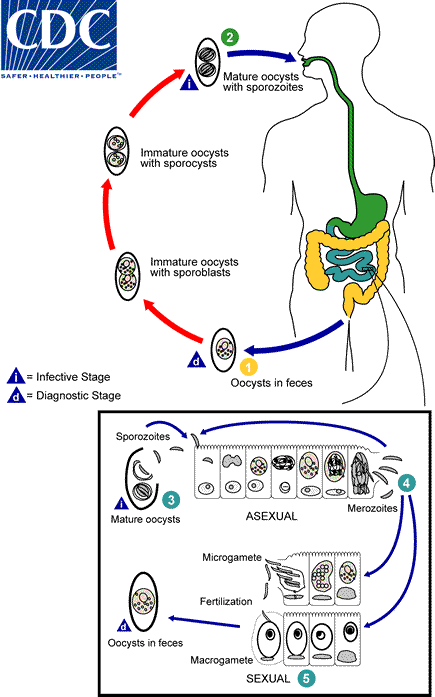
\includegraphics[width=0.85\columnwidth]{A.imagenes/ACV-BioSan-Parasit-CbelliCbios}
		\caption[Ciclo biológico y morfología de \textit{C. belli}]{Ciclo biológico y morfología de \textit{C. belli}. Vehículo: agua o alimentos contaminados, Vía: oral, Agente: Ooquiste.\label{fig:PARASIT:CbelliCBios}}
	\end{figure}
\end{multicols}
\subsubsection{Sintomatología y patogenia}
La cystoisosporosis tiene un periodo de incubación de 2 a 13 días, un periodo prepatente de 7 a 9 días y un periodo patente de 2 a 3 semanas (en pacientes inmunosuprimidos, es de 1 a 2 meses). Su principal acción patógena es la acción traumática (destruye los enterocitos y otras células intestinales). Este parásito se asocia a un gran número de eosinófilos y células plasmáticas.

La sintomatología es muy parecida a una gastroenteritis viral: febrícula, nauseas, vómitos, diarrea persistente pero autolimitantes (más de 10 deposiciones diarias), siendo estas, a veces, de aspecto grasiento y líquido, dolor abdominal y pérdida de peso. En pacientes inmunocomprometidos, las diarreas no son limitantes, y se tiende a una invasión generalizada, una isosporidosis extraintestinal, una diseminación del parásito por los ganglios linfáticos y la muerte.
\subsubsection{Diagnóstico}
La principal técnica es el diagnóstico directo por coprología, búsqueda de ooquistes en heces. Para resaltar estas formas parasitarias, se puede optar por teñir con yodo o concentrar mediante técnicas de flotación o sedimentación. Se observan en la muestras gran cantidad de cristales de Charcot-Leyden (residuos dejados por eosinófilos al entrar en apoptosis, resultado de su gran acción frente a este tipo de parásitos).
\newpage
\subsection{\textit{Cyclospora cayetanensis}}
\subsubsection{Morfología}
Considerada  una enfermedad emergente parasitaria, es de distribución cosmopolita, muy frecuente en zonas tropicales y templadas. Presenta dos formas 
\begin{itemize}[itemsep=0pt,parsep=0pt,topsep=0pt,partopsep=0pt]
	\item \textbf{Trofozoito}: tiene forma alargada, con puntas romas en sus extremos. En su polo apical presenta el complejo apical propio del phylum Apicomplexa. Bajo este se halla un pequeño citostoma (microporo). Presenta un núcleo grande con un nucléolo grande. En su citoplasma se halla un aparato de Golgi, un retículo endoplásmico y mitocondrias. Las formas de trofozoito reciben un nombre distinto según se originen de esporogonias, gamogonias,… su localización habitual es el interior del enterocito, entrando en el mediante fagocitosis inducida, disponiéndose bajo el borde en cepillo.
	\item \textbf{Ooquiste}: fase de resistencia, presenta una cubierta externa quística protectora, con un orificio taponado (micropilo), los esporoquistes y una masa de restos de las divisiones celulares, el residuo ooquistico. Una vez maduro, ese micrópilo se abre y deja salir las fases al exterior. En el interior de estos se forman los esporoquistes, unas estructuras cubiertas por una membrana con los esporozoitos en su interior (con su forma de coccidio típica) y un residuo esporoquistico. Forman 4 esporozoitos en su interior, repartidos en dos esporoquistes a razón de 2 por esporoquiste.
\end{itemize}
\subsubsection{Ciclo biológico}
\begin{multicols}{2}
	La vía de infección de \textit{Cyclospora cayetanensis} es la ingestión de ooquistes maduros en agua o alimentos contaminados. Sigue un ciclo directo, siendo eurixeno.
	
	Los ooquistes aguantan el pH estomacal, abriéndose en el intestino. Los esporozoitos que surgen del ooquistes se pegan al epitelio intestinal, fijándose, redondeándose y provocando su endocitosis y formación de una vacuola que les engloba en el interior del enterocito. En el interior de la vacuola, por esquizogonia, comienza a multiplicarse, surgiendo hasta merozoitos por esquizonte. Cuando estos merozoitos crecen, hacen estallar a la célula, reiniciando el ciclo infectivo estos merozoitos. Tras varias esquizogonias, se da una gamogonia, siendo anisogámica: en la invasión de los enterocitos, parte de los merozoitos formaran microgametocitos (16 por merozoito) y parte formaran macrogametocitos (1 por merozoito). Los microgametocitos se liberan y, si se encuentran con un macrogametocito, ocurre la fecundación, generando un cigoto que formará un ooquiste. El ooquiste inmaduro se libera al exterior del organismo, ocurriendo ahí su maduración, formando 2 esporoquistes con un residuo ooquistico, con 2 esporozoitos en su interior.
	\columnbreak
	\begin{figure}[H]
		\centering
		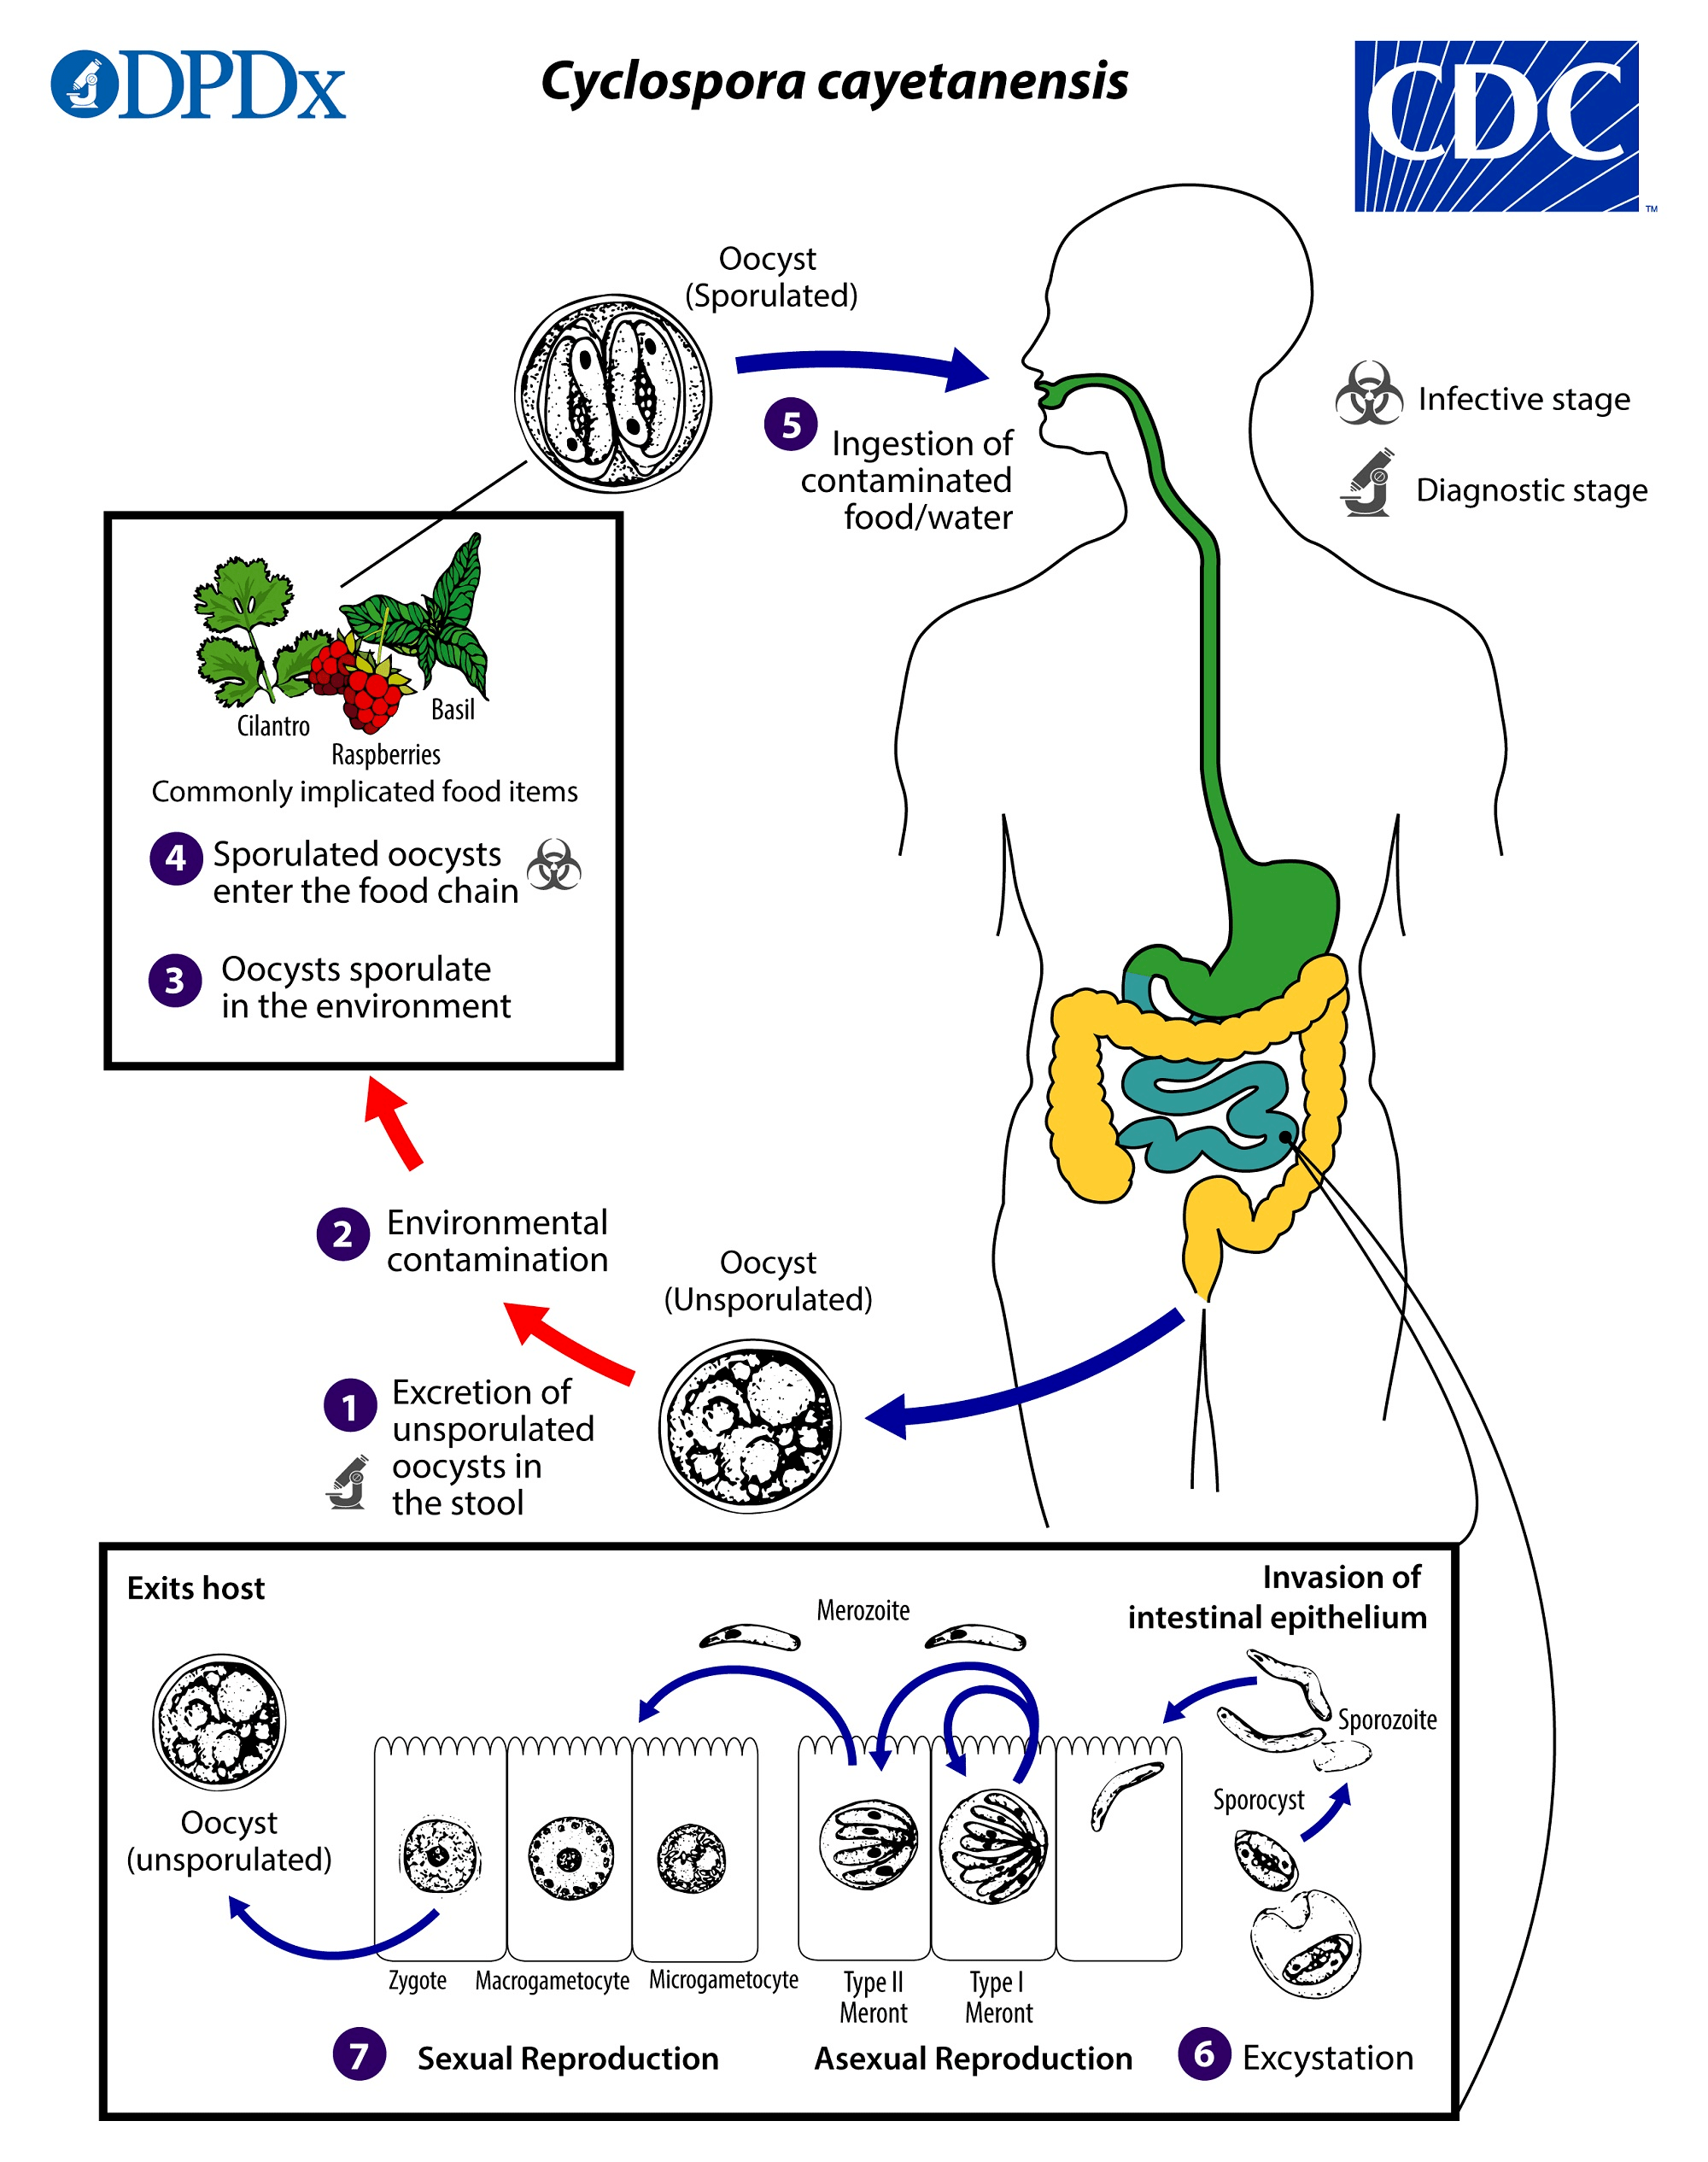
\includegraphics[width=\columnwidth]{A.imagenes/ACV-BioSan-Parasit-CcayetanensisCbios}
		\caption[Ciclo biológico y morfología de \textit{C. cayetanensis}]{Ciclo biológico y morfología de \textit{C. cayetanensis}. Vehículo: agua o alimentos contaminados, Vía: oral, Agente: Ooquiste.\label{fig:PARASIT:CcayetanesisMorf}}
	\end{figure}
\end{multicols}
\subsubsection{Patogenia y sintomatología}
La cyclosporosis provoca en el intestino una acción traumática por destrucción de las células del epitelio intestinal a la par que generan una reacción inflamatoria difusa y crónica. Todo ello genera un aplastamiento y atrofia de las vellosidades intestinales. La cyclosporosis cursa de la siguiente manera:
\begin{itemize}[itemsep=0pt,parsep=0pt,topsep=0pt,partopsep=0pt]
	\item Asintomática (se da en algunas personas, siendo portadores sanos).
	\item Sintomática, con diarreas con recaídas o cíclicas alternando con estreñimiento, pero autolimitante en inmunocompetentes, vómitos, fatiga, calambres, pérdida de peso y, en pacientes inmunosuprimidos, (VIH,…), colecistitis (por afección del conducto biliar).
\end{itemize}
\subsubsection{Diagnóstico}
La principal técnica es el diagnóstico directo por coprología, búsqueda de ooquistes en heces. Se diferencia mediante la forma y tamaño de los ooquistes (entre especies de coccidios) y por la autofluorescencia azul-verdosa bajo luz ultravioleta (característico de los coccidios).
\newpage
\subsection{\textit{Plasmodium} spp}
Paludismo, malaria o plasmodiosis son tres términos con los que se puede nombrar a la enfermedad provocada por el género de parásitos \textit{Plasmodium} spp. Estos parásitos, protozoos del phylum \textit{Apicomplexa}, familia \textit{Plasmodiidae}, presentan 5 especies capaces de infectar a los seres humanos, que son: \textit{Plasmodium vivax, P. ovale, P. falciparum, P. malariae} y \textit{P. knowlesi} (estas dos últimas parasitan al ser humano y a otros animales).
\subsubsection{Características generales}
\textit{Plasmodium} spp es un parásito que vive en la sangre, siendo un parásito intracelular de los eritrocitos. Son heteroxenos, teniendo una parte del ciclo en un hospedador intermediario (vertebrado), donde se dan procesos de esquizogonia y gametocitogénesis; y un hospedador definitivo (\textit{Anopheles}), donde se da la fecundación (final de la gamogonia) y la esporogonia. Frente a otras especies, el zigoto de este parásito es móvil, llamándose ooquineto. Todas las fases de este parásito ocurren, bien en el mosquito, bien en el vertebrado, es decir, no tiene fases de vida fuera del hospedador. Esta familia produce, por degradación de la hemoglobina, el pigmento palúdico, un pirógeno de gran importancia.

Las distintas especies se distribuyen de la siguiente forma:
\begin{itemize}[itemsep=0pt,parsep=0pt,topsep=0pt,partopsep=0pt]
	\item\textit{P. vivax}: Asia y Norte de África (34\% de casos de paludismo)
	\item\textit{P. ovale}: trópicos, EEUU, India e Indochina (poco frecuente)
	\item\textit{P. malariae}: cosmopolita (7\% de los casos)
	\item\textit{P. falciparum}: cosmopolita (50\% de los casos)
	\item\textit{P. knowlesi}: Sudeste asiático. Sin datos de prevalencia.
\end{itemize}

Antiguamente, dada la presencia de \textit{Anopheles} en las orillas del Mediterráneo, esta enfermedad también era endémica de estos países, dándose por controlada en torno a los años 60. No obstante, se han vuelto a dar casos de paludismo en estos países (Grecia, Francia, España)
\subsubsection{Morfología}
Las especies de Plasmodium presentan distintas formas celulares en su ciclo vital, que, aunque algunas son ciertamente diferentes entre las especies (teniendo valor taxonómico), son estados comunes en todas las especies. Son:
\begin{enumerate}[itemsep=0pt,parsep=0pt,topsep=0pt,partopsep=0pt]
	\item\textbf{Trofozoito}: presenta la forma típica de los \textit{Apicomplexa}, diferenciándose un estado joven, normalmente en forma de anillo; y otra madura, con una vacuola pequeña y de distinta forma.
	\item\textbf{Esquizonte}: se clasifican por el número de núcleos (merozoitos en el esquizonte maduro) que pueden presentar distintas formas.
	\item\textbf{Gametocitos}: el principal recurso para la clasificación es si deforman o no el eritrocito. 
\end{enumerate}

En cuanto a las especies, se destaca la siguiente morfología:
\begin{itemize}[itemsep=0pt,parsep=0pt,topsep=0pt,partopsep=0pt]
	\item\textit{\textbf{Plasmodium falciparum}}: responsable del 99 \% de las muertes, infectando a eritrocitos jóvenes y maduros. No presentan EES, y son proclives a causar recaídas (no se elimina totalmente al parásito, quedando a niveles que no dan síntomas). Es capaz de poliparasitar en glóbulos rojos. El trofozoito presenta forma de anillo con dos puntos de cromatina que protruyen al exterior en su fase juvenil. En su fase madura, y hasta la liberación de los merozoitos, el glóbulo rojo presenta unos gránulos, llamados de Maurer. El esquizonte (la esquizogonia dura entre 36-48 h), en su fase inmadura, almacena el pigmento palúdico en su centro. Se divide en de 8 a 32 merozoitos. El gametocito deforma el glóbulo, siendo el macho redondeado por los bordes, y el macrogametocito tiene forma de media luna.
	\item\textit{\textbf{Plasmodium vivax}}: Infecta a eritrocitos jóvenes, y realiza EES (causa de las recidivas). El trofozoito inmaduro es muy activo, presenta a veces dos puntos de cromatina y con dos anillos. El trofozoito maduro forma en el interior del hematíe unas granulaciones, los gránulos de Schuffner. La esquizogonia (de hasta 48 h) termina con entre 12 a 18 merozoitos y la hipertrofia del glóbulo rojo. El esquizonte inmaduro divide el citoplasma del eritrocito, teniendo forma irregular. El microgametocito ocupa todo el glóbulo rojo y lo no deforma, mientras que el macrogametocito es ovalado y deforma al hematíe.
	\item\textit{\textbf{Plasmodium malariae}}: No presentan EES, y son proclives a causar recaídas (no se elimina totalmente al parásito, quedando a niveles que no dan síntomas). Su parasitemia es baja, al sólo parasitar glóbulos rojos maduros. Su esquizogonia dura 72 horas.  El trofozoito tiene la forma típica de anillo, con una vacuola pequeña y el núcleo protruyendo hacia el interior. El trofozoito maduro tiene forma de prisma, y el eritrocito presenta los gránulos de Ziemann. El esquizonte inmaduro, que no deforma al hematíe, se divide en 8 merozoitos periféricos y el pigmento palúdico en el centro. Ninguno de los gametocitos deforma al glóbulo rojo, ocupándolo en su totalidad. 
	\item\textit{\textbf{Plasmodium ovale}}: Infecta a eritrocitos jóvenes, y realiza EES (causa de las recidivas). El trofozoito joven forma un anillo imperfecto, así como darse casos de poliparasitismo. En esta fase ya se encuentran presentes unos gránulos, los gránulos de Schuffer. El esquizonte acaba por formar de 6 a 12 merozoitos. Los gametocitos tienen formas redondeadas y ligeramente amorfas, deformantes del eritrocito.
	\item\textit{\textbf{Plasmodium knowlesi}}: suele parasitar simios, se confunde con otras especies por su morfología (con \textit{P. malariae}, al ser iguales sus trofozoitos maduros, y con P. falciparum, en el caso de los trofozoitos jóvenes). Su esquizogonia es la de menor duración, 24 horas (picos de fiebre diarios).
\end{itemize}
\begin{figure}[H]
	\centering
	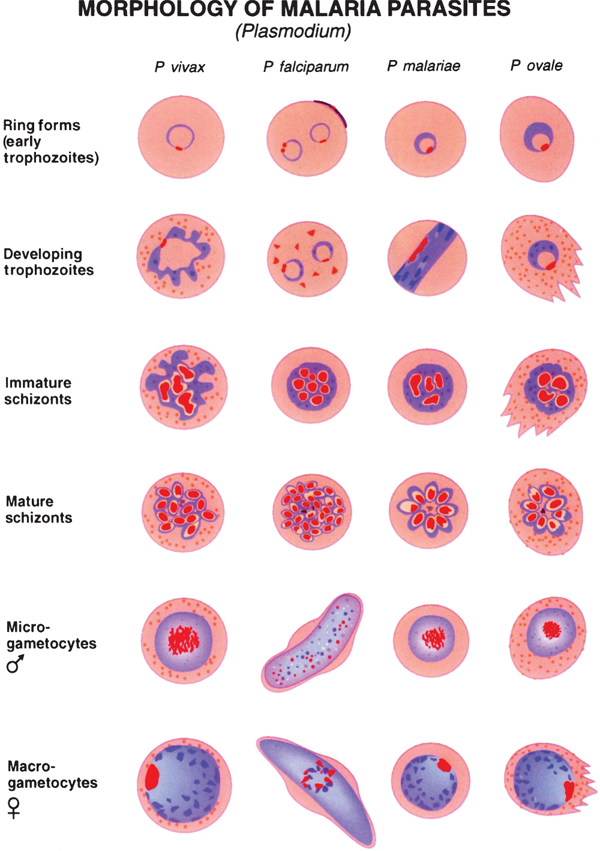
\includegraphics[trim=0 0 0 2cm,clip,width=0.75\columnwidth]{A.imagenes/ACV-BioSan-Parasit-PlasmodiumMorf}
	\caption[Morfología de las distintas especies de \textit{Plasmodium}]{Morfología de las distintas especies de \textit{Plasmodium} en las diferentes fases del parásito y su parasitación en el eritrocito, con las consecuencias de esta relación. \textit{P. falciparum} tiene poliparasitismo en su fas de trofozoito (conocido como gránulos de Maurer en esta fase), forma de 8 a 32 merozoitos deformando los eritrocitos. \textit{P. vivax} forma dos glóbulos de cromatina, y forma lo que se conocen como gránulos de Schuffner, y genera de 12 a 18 merozoitos. \textit{P. malariae} forma un nuclo no saliente y una vacuola pequeña, produciendo lo que se denominan gránulos de Zieman y forma 8 merozoitos en el eritrocito. Por último \textit{P. ovale} genera gránulos de Schuffner en su forma de trofozoito, y se forman de 6 a 12 merozoitos.}
\end{figure}
\subsubsection{Ciclo biológico}
El ciclo biológico comienza con la picadura de una hembra de \textit{Anopheles} spp parasitada inocula, junto con su saliva, esporozoitos en la sangre del hospedador intermediario. Desde la picadura, tarda unos 15 min. en llegar al hígado, entrando en los hepatocitos. En el interior de estas células, de los hepatocitos, pueden darse dos comportamientos: que \textit{Plasmodium} realice una esquizogonia (EEP: Esquizogonia Exoeritrocítica Primaria) en el hepatocito, denominada esa fase <<criptozoito>>, saliendo a posteriori al exterior cientos de merozoitos (<<metacriptozoitos>>); o que estos parásitos se queden en letargo (al hepatocito se le denomina <<hipnozoitos>>), dándose a posteriori una esquizogonia que los reactive (EES: Esquizogonia Exoeritrocítica Secundaria).

El metacriptozoito en sangre penetra en los eritrocitos (que le proporcionan un lugar de aislamiento del sistema inmune y elementos necesarios en su nutrición (hemoglobina)). En el interior de estos, toma una nueva forma, la de trofozoito, que tiene dos subfases, la de trofozoito joven, y la de maduro. Esta última, que produce el pigmento palúdico, comienza una nueva esquizogonia (el tiempo que tarda en realizar esta fase depende de cada especie), formándose el esquizonte en el interior del glóbulo rojo. Una vez que se forman los merozoitos, por presión, el eritrocito estalla, liberándolos junto con el pigmento palúdico (lo que se relaciona con los picos de fiebre de esta enfermedad: producidos por el pigmento palúdico y la propia parasitemia), pudiendo seguir estos merozoitos dos caminos: reiniciar la fase eritrocítica en otro glóbulo rojo; o comenzar una fase de gametocitogénesis en el interior de otros glóbulos rojos, diferenciándose en ellos en micro y macrogametocitos.

Cuando una hembra de \textit{Anopheles} pica a un individuo infectado, es capaz de incorporar a su interior a esos gametocitos. En su estómago, se rompen los eritrocitos y salen estos gametocitos. Los microgametocitos, por exflagelación, se transforman en microgametos; mientras que los macrogametocitos se diferencian en macrogametos. De la unión de estos, por el proceso de fecundación, continuación de la fase de reproducción sexual (gamogonia), se forma el zigoto, ooquineto. Este viaja por la pared externa del estómago, redondeándose y formando una membrana alrededor, formándose el ooquiste. Este ooquiste, por esporogonia, forma directamente esporozoitos (no hay forma intermedia de esporoquistes). Estos esporozoitos se reparten por todo el organismo del mosquito, llegando a la glándulas salivales del mosquito, pudiéndose reiniciar el ciclo con otra nueva picadura.
\begin{figure}[H]
	\centering
	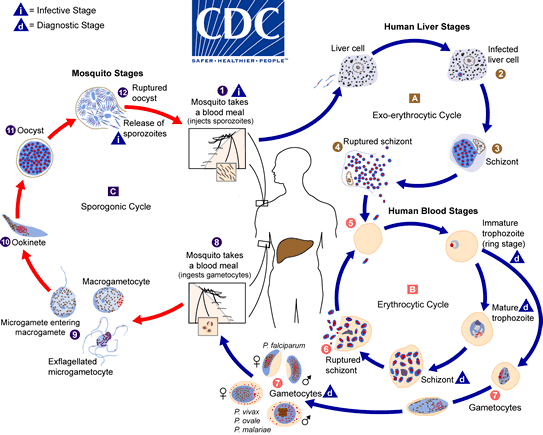
\includegraphics[width=0.85\columnwidth]{A.imagenes/ACV-BioSan-Parasit-PlasmodiumCbios}
	\caption[Ciclo vital de las distintas especies de \textit{Plasmodium}]{Ciclo vital de las distintas especies de \textit{Plasmodium}. Vector: mosquito \textit{Anopheles}. Vía: parenteral. Agente: esporozoito.}
\end{figure}
\subsubsection{Vías de transmisión}
\begin{itemize}[itemsep=0pt,parsep=0pt,topsep=0pt,partopsep=0pt]
	\item Picadura del mosquito \textit{Anopheles}, de la hembra de especies que lo puedan transmitir y que estén infectadas. Este es un riesgo presente en aeropuertos (que pasen mosquitos en el pasaje)
	\item Vía congénita (de madres no inmunes, por rotura de la placenta).
	\item Jeringuillas contaminadas
	\item Transfusiones de sangre o por trasplantes (suele ser frecuente en casos de riñón, corazón e hígado, órganos muy inervados). Este mecanismo es común en todas las especies.
\end{itemize}

En cuanto a la relación entre hospedador y parásito, se diferencian cuatro comportamientos:
\begin{itemize}[itemsep=0pt,parsep=0pt,topsep=0pt,partopsep=0pt]
	\item El parásito es incapaz de establecerse: esto ocurre en el caso de la no posesión de la proteína Duffy del eritrocito; déficit de la glucosa-6-P deshidrogenasa; talasemia; anemia falciforme o tenencia de una hemoglobina alterada.
	\item El parásito mata al hospedador: es el caso de \textit{P. falciparum}, que es mortal para personas de riesgo (inmunocomprometidos, viajeros o gente que no posee inmunidad, embarazadas, niños,$\dots$)
	\item El hospedador mata al parásito: es el caso de lactantes con madres con inmunidad frente al parasito.
	\item Parasitismo próspero o semiinmunidad: generación de portadores asintomáticos, o en fases paroxísticas.
\end{itemize}
\subsubsection{Patogenia}
Las distintas acciones que lleva a cabo el parásito son:
\begin{itemize}[itemsep=0pt,parsep=0pt,topsep=0pt,partopsep=0pt]
	\item \textbf{Traumática} de ruptura, por lisis de los eritrocitos.
	\item \textbf{Expoliadora} específica, al capturar la hemoglobina de los glóbulos rojos.
	\item \textbf{Tóxica}: genera fiebre por la propia parasitemia y por la liberación del pigmento palúdico.
	\item \textbf{Mecánica}: bloquea los capilares sanguíneos por la adsorción por parte de todo tipo de eritrocitos (sanos o infectados) que los hace propensos a pegarse en los capilares
\end{itemize}

La presencia de antígenos solubles en suero provocará una reacción inmune exagerada que se manifestará en forma de una respuesta inflamatoria exagerada, una inmunopatología. Así mismo, esos antígenos presentes en los eritrocitos, estén sanos o infectados, provocará una reacción de lisis de los mismos por acción de células del sistema inmune.

La enfermedad provocada por \textit{Plasmodium}, generará dos tipos de daños: los producidos por el parásito en su ciclo biológico, y los generados por la repuesta inflamatoria exagerada (escalofríos, fiebre, procesos autoinmunes). Así, se diferencian dos tipos de malaria: malaria no complicada (malestar con fiebre y síntomas inespecíficos) y malaria severa (que lleva a la muerte si un rápido diagnóstico).

En cuanto a los periodos de incubación, patente y prepatente, se existen diferencias entre las especies:
\begin{itemize}[itemsep=0pt,parsep=0pt,topsep=0pt,partopsep=0pt]
	\item\textbf{Periodo de incubación}: puede ir desde los 7 días (\textit{P. falciparum}); 18 días (\textit{P. vivax, P. ovale}) o hasta 42 días (\textit{P. malariae})
	\item\textbf{Periodo patente}: es de 8 días en todas las especies, excepto \textit{P. malariae}, que es de 17 a 37 días.
	\item\textbf{Periodo patente}: el lapso puede ser desde 1.5 años (\textit{P. falciparum}); 5 años (\textit{P. vivax, P. ovale}) o hasta 30 años (\textit{P. malariae}). En casos de malaria severa, puede ser de entre 28 y 42 días, dependiendo de la especie.
\end{itemize}

Según los síntomas, la malaria tiene dos fases diferenciables, que se explican según el ciclo vital del parasito. Estas son:
\begin{itemize}
	\item \textbf{Fase exoeritrocítica}: acontece la multiplicación de \textit{Plasmodium} spp. en el interior de los hepatocitos. Dura de 8 a 42 días, según la especie, y es una fase asintomática.
	\item\textbf{Fase eritrocítica}: es la fase de multiplicación del metacriptozoito en el interior del glóbulo rojo. La destrucción de los eritrocitos conlleva a una anemia (descenso de los niveles de hierro y hemoglobina) y una hipertrofia del bazo en pos de aumentar el número de células sanguíneas. En los casos de paludismo por \textit{P. falciparum}, existe, por un proceso de eritrofagocitosis provocada por la adsorción de antígenos solubles a la membrana plasmática de glóbulos rojos sanos y parasitados, un bloqueo de microcapilares, que puede desembocar en una trombosis cerebral.
	La hemoglobina libre, que se metaboliza en bilirrubina que provoca un daño hepático al metabolizarla en el hígado, apareciendo la ictericia. Esto, la bilirrubina, junto con el pigmento palúdico, que tiende a acumularse en hígado, bazo y cerebro, provoca graves brotes de fiebre de aparición cíclica. La destrucción de los eritrocitos y liberación de hemoglobina provoca una anoxemia (descenso del O$_2$ en sangre) y con ello, una hipoxia en todos los órganos y tejidos, provocando daño suprarrenal, hepático, esplénico, gastrointestinal (otro síntoma de malaria pueden ser heces con sangre o vómitos con sangre), cerebral y pulmonar.
\end{itemize}
\subsubsection{Sintomatología}
El paludismo se caracteriza por manifestarse en fases asintomáticas y sintomáticas, por lo que se le nombró en un principio como <<fiebres tercianas>> (ciclos de 48 días) o <<fiebres cuartanas>> (ciclos de 72 horas). Estas fases con sintomatología se denominan ataque palúdico, fases paroxísticas de la enfermedad con elevaciones bruscas de la temperatura. Duran de 8 a 12 horas y comienzan de la siguiente forma:
\begin{enumerate}[itemsep=0pt,parsep=0pt,topsep=0pt,partopsep=0pt]
	\item El enfermo comienza a sentir un frío intenso, escalofríos y comienza a subirle la temperatura.
	\item Cuando la fiebre llega a los 40 o hasta 42ºC, se dan síntomas de delirio, nauseas, vómitos y fortísimas convulsiones.
	\item Se da un periodo de intensa sudoración y una bajada de la fiebre, que dura unas 2 ó 3 horas.
	\item El paciente se duerme y se despierta sin ningún malestar.
\end{enumerate}

Estos ataques palúdicos pueden empezar con ciertos síntomas previos (febrículas, malestar,etc. síntomas vagos) o tener un inicio brusco. Cada ataque palúdico coincide con un ciclo de esquizogonia en el glóbulo rojo. Estas fases se repetirán, dependiendo de la especie, cada 24 (\textit{P. knowlesi}), 48 (\textit{P. vivax, P. ovale, P. falciparum}) o 72 horas (\textit{P. malariae}).

Una de las especies de Plasmodium más agresivas es \textit{P. falciparum}, del cual se deben mencionar dos clases de paludismo especial asociados a este parásito:
\begin{itemize}[itemsep=0pt,parsep=0pt,topsep=0pt,partopsep=0pt]
	\item \textbf{Paludismo cerebral}: conduce a la muerte en poco tiempo, si no hay un rápido tratamiento. Sus síntomas son: ceguera, epilepsia, ataque renal, esplenomegalia enorme, hepatomegalia e ictericia, cefalea progresiva hasta llegar al coma y fiebre superior a los 42ºC.
	\item \textbf{Paludismo congénito}: es raro, y el más asociado a esta patología es \textit{P. falciparum}. Aparece cuando la placenta está dañada (generalmente es el propio parasito el que rompe la placenta) y se adquiere en el momento del parto. Es muy frecuente en madres no inmunes, por el curso más severo de la enfermedad en ellas, que afecta a la placenta.
\end{itemize}
\subsubsection{Inmunidad}
La semiinmunidad se relaciona con una exposición intensa y prolongada en áreas de malaria endémica, con una transmisión persistente. Así mismo, esta se desarrolla de forma lenta, en torno a 5 ó 10 años, siendo esta no permanente (se puede perder cuando el individuo semiinmune deja de estar expuesto). Mantiene la enfermedad de forma asintomática, protege frente a la malaria severa, pero no evita la infección, dejándola a niveles submicroscópicos, apenas detectables, pero que los hace transformarse en portadores asintomáticos.

En cuanto a la respuesta inmune, la parasitemia provoca la producción de IgG y de la estimulación de linfocitos T CD4 y CD8 en sangre e hígado respectivamente. Esta última es el tipo de inmunidad (la inmunidad celular) la más efectiva cuando \textit{Plasmodium} está en el interior de la célula.
\subsection{Diagnóstico}
Se pueden llevar a cabo las siguientes técnicas:
\begin{itemize}[itemsep=0pt,parsep=0pt,topsep=0pt,partopsep=0pt]
	\item \textbf{Diagnóstico etiológico}: mediante análisis de sangre, se puede localizar mediante dos técnicas:
	\begin{itemize}
		\item Por frotis teñidos con Giemsa (tan solo se localizan en concentraciones mayores a los 5 o 16 parásitos/$\mu$L)
		\item Por gota gruesa: se depositan tres gotas de sangre sobre un porta (técnica de concentración), remover en un área de unos 2 cm$^2$ durante 30 segundos para desfibrinar, secar y limpiar. Posteriormente se tiñe con Giemsa sin fijar con metanol.
	\end{itemize}
	\item \textbf{Diagnóstico indirecto}: ya sea mediante técnicas serológicas (IFI,$\dots$) o por tiras cromatográficas reactivas, inmunocromatografía (útiles en campañas epidemiológicas por su rapidez y bajo coste)
	\item \textbf{PCR}: de gran sensibilidad y especificidad (cercanas al 100\%), identifican la especie, así como permiten diagnosticarlo cuando se hallan en concentraciones muy bajas (hasta 0.002 parásitos/$\mu$L).
\end{itemize}
\newpage
\subsection{\textit{Toxoplasma gondii}}
Toxoplasma gondii es un parásito del filo \textit{Apicomplexa} con distribución cosmopolita, que varía su prevalencia e incidencia según las costumbres culinarias de la zona. Es más incidente en aquellas zonas donde es costumbre cocinar poco la carne, mientras que en zonas donde es costumbre hacerlo en gran medida, es poco común.

El parásito fue descubierto en 1908, en 1937 fue descrita su transmisión congénita, pero hasta 1965 no se supo todas las fases y hospedadores de su ciclo vital.
\subsubsection{Morfología}
Según su estado de desarrollo, se diferencian tres estados:
\begin{itemize}[itemsep=0pt,parsep=0pt,topsep=0pt,partopsep=0pt]
	\item \textbf{Esporozoitos}: taquizoitos con mayor número de rotrias y micronemas. Surgen por esporogonia. Contenidos dentro de los ooquistes (uno en los inmaduros,  dos en los maduros), la maduración de estos ooquistes acontece en el exterior. Se destruyen con calor.
	\item \textbf{Taquizoitos}: originados por endopoligenia, tienen una morfología muy similar a la del coccidio típico. No resisten la digestión en el estómago, pero se multiplican rápidamente. Con forma de media luna, tras la multiplicación por endopoligenia, se multiplican rápidamente y se diseminan por el organismo. Son capaces de atravesar la placenta.
	\item \textbf{Bradizoitos}: surgen por endodiogenia, proceso más lento, son las formas presentes en infecciones crónicas, dado que son las formas que se hallan en los quistes tisulares de \textit{T. gondii}. Resisten la digestión, no se activan salvo inmunosupresión. No son capaces de sobrevivir a temperaturas de más de 65º o menores a -20ºC.
\end{itemize}
\begin{figure}[H]
	\centering
	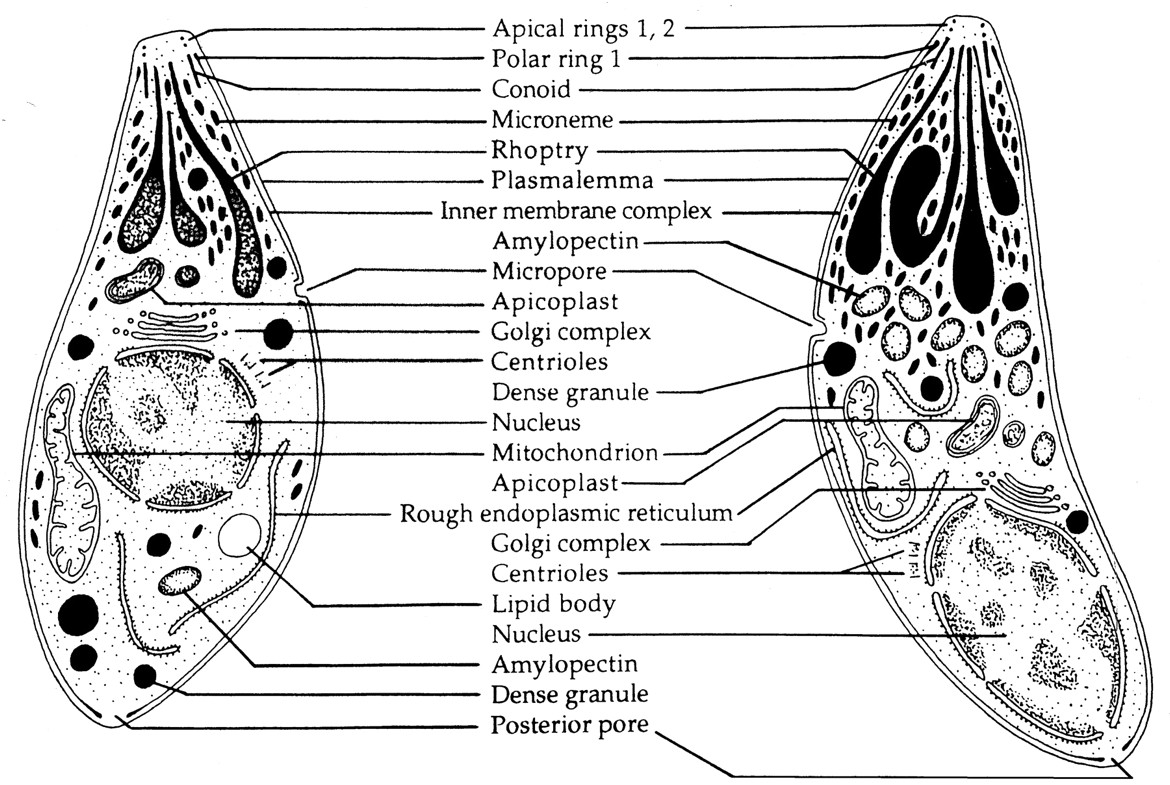
\includegraphics[width=0.7\columnwidth]{A.imagenes/ACV-BioSan-Parasit-TgondiiMorf}
	\caption[Morfología de \textit{T. gondii}]{Comparativa de las formas de taquizoito y bradizoito de \textit{T. gondii}.}
\end{figure}
\subsubsection{Ciclo biológico}
El ciclo comienza tras la gamogonia, en el intestino del hospedador definitivo, el gato. Tras este proceso de reproducción sexual, comienza la esporogonia, saliendo al exterior los ooquistes inmaduros. De 1 a 5 días, de un esporozonte se obtienen dos esporoquistes, con 4 esporozoitos cada uno y el residuo esporoquistico. Estos esporozoitos son infectantes para todos los hospedadores. 

Los hospedadores intermediarios se infectan, bien por la ingesta de ooquistes maduros como a partir de la ingesta de bradizoitos presentes en carnes contaminadas, pasando al intestino delgado. Allí, penetran y se dirigen al endotelio de los capilares sanguíneos por un proceso de endopoligenia. Así, se forman taquizoitos, que se dispersan por los tejidos, infectando a las células, introduciéndose dentro de una vacuola. A esa célula infectada se le denomina pseudoquiste. Allí, por endopoligenia, se forman más taquizoitos, que, tras muchas multiplicaciones, hacen estallar la célula y se liberan. Así, continúan durante 3 semanas, tras las cuales surge una respuesta inmune, momento en el que el parásito se queda confinado a células nerviosas, del ojo y fibras musculares, donde, por endodiogenia, se multiplica y transforma en bradizoitos. El consumo por parte de otro hospedador dará lugar a una reiniciación del ciclo o, en el gato, la terminación del ciclo.

Estos <<zoitos>>, en el gato (pasan por consumo de carne contaminada (ratones, fundamentalmente) se reproducen, en los enterocitos del intestino delgado del gato por endopoligenia, endodiogenia y esquizogonia. Los merozoitos que surgen de este último proceso, la esporogonia, comienzan la reproducción sexual: la gamogonia. Una serie de células en microgametocitos, otras células, en macrogametocitos. Tras la fecundación, se obtiene un zigoto que forma el esporonte del ooquiste inmaduro.

La infección en el gato dependerá de la forma parasitaria que ha ingerido. La forma de esporozoito tiene un periodo prepatente de unos 20 días. Los taquizoitos, de menos de 19 días, y los quistes, de 3 a 10 días. También es importante señalar la importancia de una vía congénita de transmisión del parásito, solo posible cuando está en fase de taquizoito (antes de la inmunidad).
\begin{figure}[H]
	\centering
	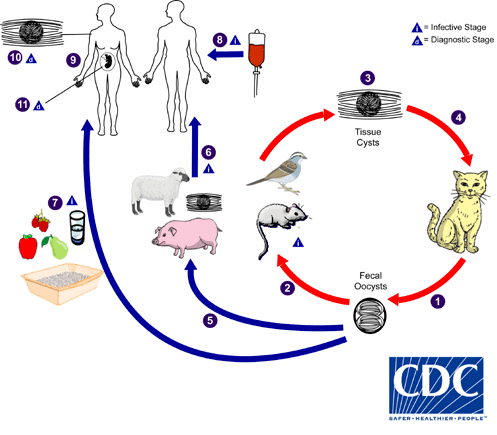
\includegraphics[width=0.7\columnwidth]{A.imagenes/ACV-BioSan-Parasit-TgondiiCbios}
	\caption[Ciclo biológico de \textit{T. gondii}]{Ciclo biológico de \textit{T. gondii}.Vehículo: agua o alimentos contaminados, Vía: oral, parenteral o placentaria, Agente: cualquier fase. El único hospedador definitivo conocido es miembros de la familia \textit{Felidae}. (1): los ooquistes no esporulados salen de las heces del gato. Aunque estos tardan de 1 a 2 semanas en madurar, se generan en gran cantidad. Tras 1 o 5 días, los ooquistes maduran en el ambiente, comenzando a ser infecciosos. Los hospedadores intermedios naturales (pájaros y roedores) se infectan por agua o alimentos contaminados. (2 y 3): los ooquistes se transforman en en taquizoitos, que se localizan en tejidos nervioso y muscular y se transforman en bradizoitos. (4): Los gatos se infectan por la ingestión de estos hospedadores infectados, repitiendo el ciclo. Los seres humanos se infectan, siendo un hospedador intermedio no esperado, infectandos por la ingestión de carne contaminada con el parásito (5 y 6); alimentos contaminados (7), transfusiones y via placentaria (8 y 9). En el ser humano, el parásito repite el patrón de los hospedadores intermedios, pero nunca terminará el ciclo.}
\end{figure}
\subsubsection{Vías de transmisión y control}
Para el hospedador intermedio (el hospedador definitivo se contagia por el consumo de carne contaminada con bradizoitos, normalmente, aunque las tres fases le resultan infectantes), se transmite:
\begin{itemize}[itemsep=0pt,parsep=0pt,topsep=0pt,partopsep=0pt]
	\item \textbf{Ingestión} de carne poco cocinada contaminada con quistes con bradizoitos.
	\item \textbf{Ingestión} de agua o verduras con ooquistes maduros (esporozoitos).
	\item \textbf{Transfusiones}, vía trasplacentaria o durante la lactancia (taquizoitos).
\end{itemize}

Así, los elementos de control son:
\begin{itemize}[itemsep=0pt,parsep=0pt,topsep=0pt,partopsep=0pt]
	\item Rápida eliminación de heces de gatos.
	\item Limpieza de vegetales crudos.
	\item Guantes para manipular heces.
	\item Cocinado de los alimentos a más de 66º o congelación a menos de -20º.
	\item Diagnóstico precoz en el embarazo (importantes son los títulos límite de infección aguda y crónica y/o diagnóstico con IgM (de fases crónicas)).
\end{itemize}
\subsubsection{Patogenia y sintomatología}
El periodo de incubación de la toxoplasmosis es de 2 días, el periodo prepatente dura desde varios días a semanas, y el periodo patente se extiende durante años. 

La principal acción de \textit{Toxoplasma gondii} suele ser acción traumática por destrucción de las células que infecta (pseudoquistes) y se desarrolla. Suele cursar asintomática por lo general, dado que esa destrucción se ve compensada por la regeneración celular.

Así, la enfermedad cursa según dos periodos:
\begin{enumerate}[itemsep=0pt,parsep=0pt,topsep=0pt,partopsep=0pt]
	\item \textbf{Toxoplasmosis aguda}: se manifiesta por una linfoadenopatía de los ganglios cervicales (90\% de los casos), siendo estos duros y dolorosos. Esta linfoadenopatía se acompaña de fiebre, malestar general, cansancio, dolores musculares y de cabeza. En algunos casos, la patología se complica con afecciones del SNC (4.3\%), miocarditis (1.4\%) y neumonía (0.8\%).
	\item \textbf{Toxoplasmosis crónica}: a las tres semanas de la infección crónica, comienza la fase crónica, con un desarrollo de la inmunidad frente a este parásito, pero que no le erradica. Esta fase dura meses o años. Es un periodo asintomático, en el que los quistes con bradizoitos no son nocivos salvo reactivaciones (pacientes inmunosuprimidos) que produzcan la rotura de los quistes y la liberación de los bradizoitos. La multiplicación de los bradizoitos origina focos de necrosis e inflación, provocando, en la retina, ceguera, o fallos en distintos órganos y, por ello, muerte.
\end{enumerate}

La toxoplasmosis también puede transmitirse por vía congénita (toxoplasmosis congénita o  subaguda). Por vía placentaria llega hasta el feto, desarrollándose de forma anómala. La tasa de infección a medida que avanza el embarazo es inversamente proporcional a los daños producidos en el feto. Así, durante el primer trimestre, tan solo se infecta el 14\% de los expuestos, cursando con daños letales al feto y abortos. En el segundo, esa tasa es del 29\%, y en el tercero, del 59\%. En estos casos, los daños no son letales, pero provocan ciertos problemas neurológicos. Así, \textit{T. gondii} causa los siguientes daños: hidrocefalia, problemas neurológicos, esplenomegalia, hepatomegalia, calcificaciones en el SNC, convulsiones.
\subsubsection{Diagnóstico}
Dada la imposibilidad de realizar un diagnóstico directo, se realizan las siguientes pruebas:
\begin{itemize}[itemsep=0pt,parsep=0pt,topsep=0pt,partopsep=0pt]
	\item \textbf{Dye-test} o \textbf{Técnica de Sabin-Feldman}: para ella se usan \textit{T. gondii} vivos, a los que se les cultiva con el suero problema (se busca saber si hay anticuerpos contra \textit{T. gondii} en él, indicativo de presencia) y azul de metileno a 37ºC durante 30 minutos. Se estudia morfología (el parásito se deforma si es positivo a la presencia de anticuerpos), movilidad (positivo si son inmóviles) y sensibilidad a la tinción (si es positivo, no se colorean).
	\item \textbf{Inmunodiagnóstico}: sin riesgo de manipulación, se hace mediante técnicas de IFI, ELISA, HAI, pudiéndose además obtener datos cuantitativos. Dado que la evolución de los anticuerpos es la de repetir una campana de Gauss, los datos pueden tomarse de forma errónea en métodos cuantitativos, se recomienda, una vez realizada la medición, o repetirla a los 21 días, o realizarla con anti-IgM, que indican curso agudo y no pueden atravesar la placenta. Así mismo, se ha de contar con que \textit{T. gondii} posee autofluorescencia azul, luego se ha de eliminar mediante la adición de azul Evans, que enmascara esa característica.
	\item \textbf{Aislado y cultivo} (necropsias).
	\item\textbf{PCR}
\end{itemize}
\newpage
\subsection{\textit{Eimeria}}